\part{APÉNDICES}
\chapter{KIT de supervivencia para Matemáticas - 2} \label{Kit}


Lo que debes saber antes de empezar a estudiar Matemáticas de ciencias en segundo de bachillerato.

\section{Aritmética y Álgebra}

\begin{multicols}{2}

$(a \pm b )^2=a^2 \pm 2 a b + b^2$ 

$(a+b)(a-b)=a^2-b^2$

$(a+b+c)^2 = a^2+b^2+c^2+2ab+2ac+2bc$

$(a+b)^3 = a^3 + 3a^2b + 3ab^2 +b^3 $

$(a+b)^n= \left(\begin{matrix}n\\0\end{matrix}\right) a^n + \left(\begin{matrix}n\\1\end{matrix}\right)a^{n-1}b + \left(\begin{matrix}n\\2\end{matrix}\right) a^{n-2}b^2+ \cdots + \left(\begin{matrix}n\\n-1\end{matrix}\right)a b^{n-1}+ \left(\begin{matrix}n\\n\end{matrix}\right)b^n=\sum _{ k=0 }^{ n }{ \left( \begin{matrix} n \\ k \end{matrix} \right)   a^k b^{n-k} }  \quad  $. 

\emph{Binomio de Newton}

 	\begin{figure}[H]
		\centering
		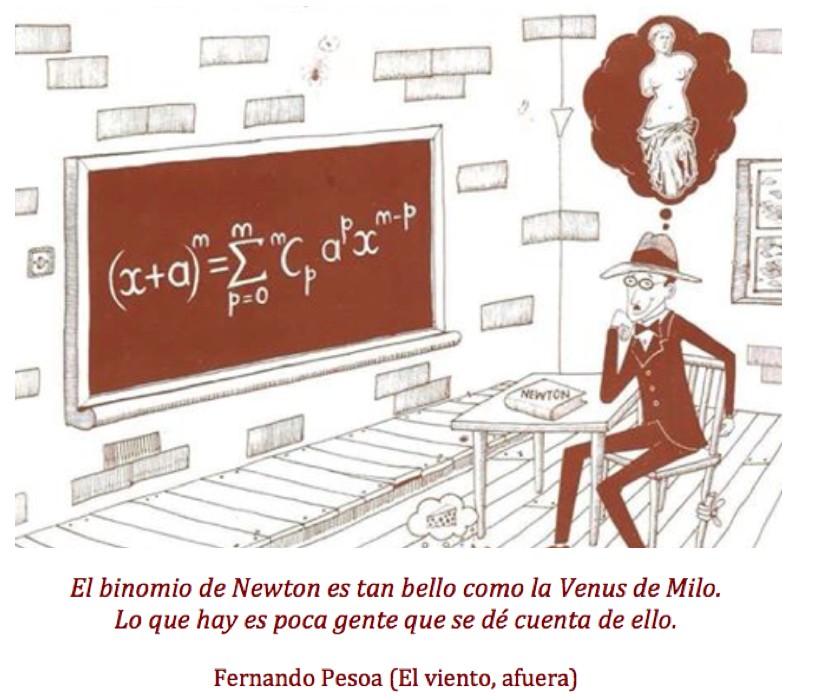
\includegraphics[width=.4\textwidth]{imagenes/apendices/APENDICESIM01.png}
		\caption {El poeta Fernando Pesoa admirando el binomio de Newton.}
	\end{figure}
\end{multicols}

PROGRESIONES ARITMÉTICAS Y GEOMÉTRICAS:

PA: $a_n=a_1+(n-1)d; \quad S_n=\dfrac {a_1+a_n}{2}\; n$

PG: $a_n=a_1 \; r^{n-1}; \quad S_n=\dfrac{a_n\cdot r-a_1}{r-1 }; \quad \mbox{ si } |r|<1 \to S_{\infty}=\dfrac {a_1}{1-r}$

POTÉNCIAS Y RAÍCES:

$a^0=1 \; (a\neq 0); \quad  a^{-n}=\dfrac {1}{a}; \quad  (ab)^n=a^n\; b^n; \quad \left( \dfrac {a}{b} \right)^n=\dfrac {a^n}{b^n}$

$a^m\cdot a^n=a^{m+n}; \quad \dfrac {a^m}{a^n}=a^{m-n}; \quad (a^m)^n=a^{m\cdot n}; \quad a^{\dfrac m n}= \sqrt[m]{a^m}$

$\sqrt[m]{\sqrt[n]{x}}=\sqrt[m\cdot n]{x}; \quad \sqrt[m]{xy}=\sqrt[m]{x}\;\sqrt[m]{y}; \quad \sqrt[m]{\dfrac {x}{y}}=\dfrac {\sqrt[m]{x}}  {\sqrt[m]{y}}$

Recordad las técnicas de racionalización.

LOGARITMOS:

$a>0; \; a\neq 1: \quad \mathrm{log}_a (x)=y \leftrightarrow y=a^x; \; y\in\mathbb{R^+_*}\; \; $ Es la función inversa a la exponencial.

Propiedades de la función logarítmica:

La función logarítmica es inyectiva: $x_1\neq x_2 \to \mathrm{log}_a x_1 \neq \mathrm{log}_a x_2$
\begin{multicols}{2}

$\mathrm{log}_a a=1; \qquad \mathrm{log}_a 1=0$

$\mathrm{log}_a (x_1\cdot x_2)=\mathrm{log}_a x_1+\mathrm{log}_a x_2$

$\mathrm{log}_a \left( \dfrac {x_1}{x_2} \right)=  {\mathrm{log}_a x_1}-{\mathrm{log}_a x_2} $

$\mathrm{log}_a x^n=n\cdot \mathrm{log}_a x$

$\mathrm{log}_a \sqrt[n]{x}= \dfrac 1 n \mathrm{log}_a x$


	\begin{figure}[H]
		\centering
		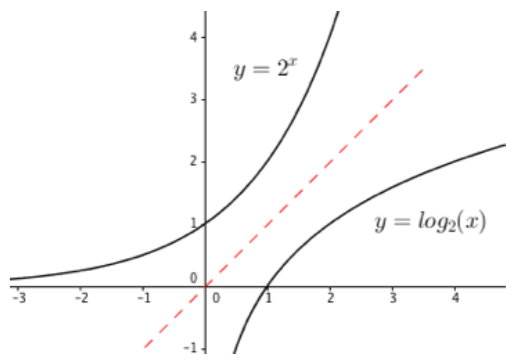
\includegraphics[width=.3\textwidth]{imagenes/apendices/APENDICESIM02.png}
		\caption {Funciones exponencial y logarítmica}
	\end{figure}
\end{multicols}

Cambio de base en la función logarítmica: $\mathrm{log}_a x = \dfrac {\mathrm{log}_b x}{\mathrm{log}_b a}$

Logaritmos más usuales:  

$* \quad$ si $a=10$, tenemos los logaritmos decimales, muy usados en química (ph), se suelen escribir como $\mathrm{log}_{10} x = \mathrm{Log} x$

$* \quad$ si $a=e$, tenemos los logaritmos neperianos  o naturales, son los más usuales en ciencia por su sencillez (inversa de $e^x$) tanto en cálculo diferencial como integral. Su notación suele ser $\mathrm{log}_e x= \mathrm{log} x =\mathrm{ln} x$

\textit{En muchas ocasiones se nos presentan funciones exponenciales de bases distintas a $e$, también podemos cambiar de base en la función exponencial: $y=a^x$, tomemos $\mathrm{ln}\;$ : $\mathrm{ln}y=x\cdot \mathrm{ln} a$. Despejando: $y=e^{ x\cdot \mathrm{ln} a } \quad \Rightarrow \quad a^x=e^{  \mathrm{ln} a \cdot x}$ }

POLINOMIOS:

Se llama \emph{raíz} de un polinomio a aquellos valores de la variable $x$ para los cuales el el valor numérico del polinomio es cero: $a$ raíz de $p(x) \leftrightarrow p(a)=0$

Las siguientes expresiones tienen el mismo significado:


	\hspace{10mm}  $p(a)=0$
	
	\hspace{10mm}  $p(x)$ es divisible por $(x-a)$
	 
	 \hspace{10mm} $a$ es raíz de $p(x)$
	 
	 \hspace{10mm} $(x-a)$ divide a $p(x)$
	 
	 \hspace{10mm} Encontrar las raíces de $p(x)$ es resolver la ecuación $p(x)=0$

Si un polinomio de segundo grado tiene como raíces $x_1$ y $x_2$, se podrá factorizar como: $\textbf{a} x^2+bx+c=\textbf{a}\cdot (x-x_1) \cdot (x-x_2)$

Para factorizar un polinomio, encontrar sus raíces (racionales), usamos la `Regla de Ruffini' aplicando la regla de Cardano-Vieta: las posibles raíces de $p(x)$ han de ser cocientes en que el numerador sea un divisor del término independiente y el denominador divisor del término dominante (de mayor grado).

ECUACIONES:

$\circ \quad$ Ecuaciones de primer grado: $ax=b \to x=-b/a$

$\circ \quad$ Ecuaciones de segundo grado: $a x^2 + b x +c =0 \to x =\dfrac {-b \pm \sqrt{b^2 - 4ac}}  {2a}$ ; esta es la llamada fórmula general. Si la ec. es incompleta (siempre con $a \neq 0$ se pueden resolver, más rápidamente, despejando o sacando factor común.

$\circ \quad$ Ecuaciones reducibles a segundo grado (generalización de las `bicuadradas'): $a x^{2n} + b x^n + c = 0$, aparece la variable elevada a dos potencias, una doble que la otra. En estos casos, el cambio de variable $x^n=t; \; x^{2n}=t^2$ conduce la ecuación inicial a una de segundo grado siendo $t$ la incógnita: $a t^2 + b t+ c =0$, que se resuelve y, !`atención!, hay que recordar \emph{deshacer el cambio de variable} establecido. P.e., si $t_1$ fuese una solución de la última ecuación resuelta (segundo grado en $t$), ahora tendríamos $x^n=t_1 \to x=\sqrt[n]{t_1}$

 $\circ \quad$ Ecuaciones polinómicas (grado mayor o igual a tres). Hay que factorizar el polinomio por Ruffini u buscar las raíces o soluciones. 

$\circ \quad$ Ecuaciones racionales (sobre fracciones algebráicas). Al multiplicar `toda la ecuación' por el `mcm de los denominadores', desaparecen todos y tenemos una ecuación polinómica que habrá que resolver. Al haber multiplicado la ecuación inicial por un polinomio (mcm),  podría ocurrir que una de las soluciones obtenidas de la ecuación polinómica fuese raíz del mcm y hubiésemos multiplicado nuestra ecuación original por cero, lo cual no tiene ningún sentido, para asegurarnos de que esto no ocurre bastará con: \emph{!`En las ecuaciones racionales es NECESARIO comprobar que las soluciones obtenidas no anulen ningún denominador de la ecuación original.!}

$\circ \quad$ Ecuaciones irracionales (con la incógnita bajo alguna raíz cuadrada). Aislaremos la raíz en un solo miembro de la ecuación y elevaremos al cuadrado. !`Cuidado: al elevar al cuadrado una ecuación, pueden aparecer soluciones extrañas!: $x=2 \to x^2=4 \to x=2 \quad \vee \quad \cancel{x=-2}$, cuya última solución no es válida, evidentemente, pues al sustituir en la ecuación original conduce a un error ($2=-2$). Luego, \emph{!`en las ecuaciones irracionales es `necesario' comprobar las soluciones obtenidas al elevar al cuadrado em la ecuación original!}. En ocasiones, si aparecen más de una raíz cuadrada, caldrá repetir el proceso de aislar la raíz en un solo término de la ecuación y elevar al cuadrado.

$\circ \quad$ Ecuaciones exponenciales, la $x$ aparece en el exponente de alguna potencia. Si se pueden aislar y agrupar en los dos miembros de la ecuación las partes con y sin incógnitas, podemos hacer uso de la propiedad inyectiva de la función exponencial ($a^x=a^k \leftrightarrow x=k$). En caso de aparecer sumas y/o restas de potencias en que aparezca la incógnita no podremos agrupar (haciendo uso de las propiedades de las potencias) y será necesario establecer un `cambio de variable', llamaremos $t$ al exponente más la incógnita más sencilla. \emph{!`Hay que recordar deshacer el cambio de variable!}

$\circ \quad$ Ecuaciones logarítmicas ($x$ dentro de algún logaritmo). Usaremos las propiedades de los logaritmos para compactar los dos términos de la ecuación solo con un logaritmo cada una y usaremos la propiedad de inyectividad de la función logarítmica. \emph{!`en las ecuaciones logarítmicas es `necesario' comprobar las soluciones obtenidas en la ecuación original!}

$\circ \quad$ Ecuaciones en valor absoluto. Se repasan en el capítulo \ref{preliminares} Preliminares, sección \ref{preliminares-ejercicios} de ejercicios.

\section{Complejos}
\begin{multicols}{2}
$i=\sqrt{-1}; \; i^2=-1; \; i^3=-i; \; i^4=1;  \qquad z\in \mathbb{Z}:\; z=a+bi\; $ Forma binómica.

$a=\mathrm{Re}(z); \; b= \mathrm{Im}(z); \quad \overline{z}=a-bi  ; \quad |z|=r=+\sqrt{z\cdot \overline{z} }; \quad \theta=\arctan \dfrac b a  \to \qquad z\in \mathbb{Z}:\; z=r_{\theta}\; $ Forma polar.

\begin{figure}[H]
		\centering
		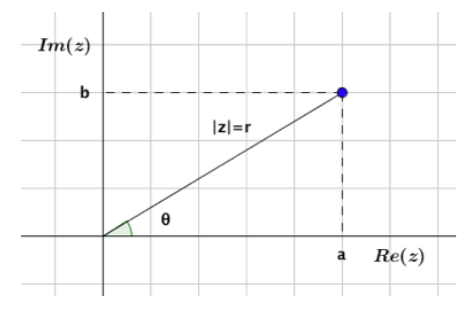
\includegraphics[width=.4\textwidth]{imagenes/apendices/APENDICESIM03.png}
	\end{figure}
\end{multicols}

Se demuestra que en $\mathbb{Z}$, cualquier ecuación polinómica de orden $n$ tiene exactamente $n$ soluciones (aunque algunas puedan ser múltiples).

Si $z=a+bi$ es una solución de una ecuación de segundo grado, también lo será su compleja conjugada $\overline{z}=a-bi$
 
\section{Trigonometría}

	\begin{figure}[H]
		\centering
		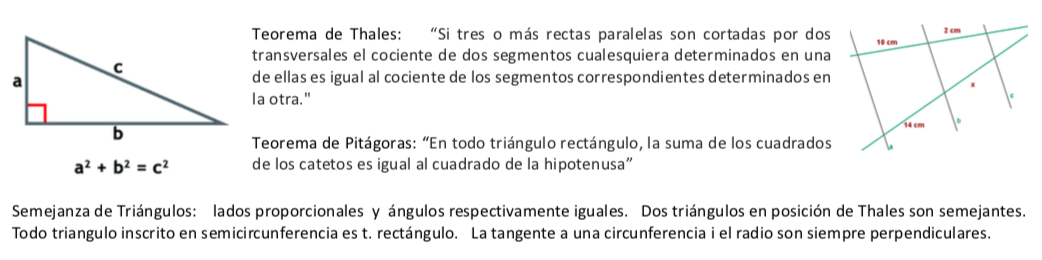
\includegraphics[width=1\textwidth]{imagenes/apendices/APENDICESIM04.png}
	\end{figure}

	\begin{figure}[H]
		\centering
		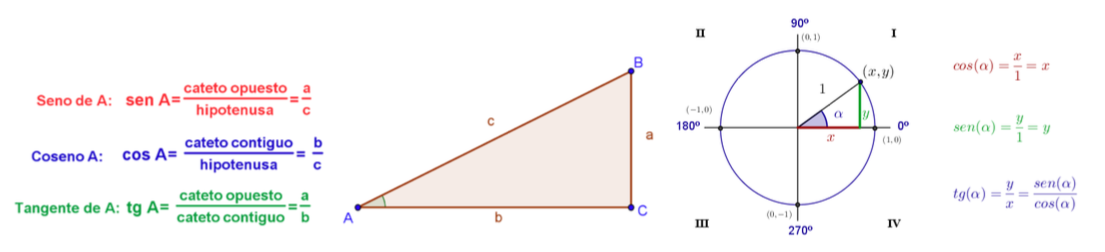
\includegraphics[width=1\textwidth]{imagenes/apendices/APENDICESIM05.png}
	\end{figure}

RELACIONES FUNDAMENTALES:

$\sin^2 x + \cos^2 x = 1 \to \tan^2 x + 1 = \dfrac {1}{\cos^2 x} \Rightarrow \begin{cases}
 	\sin^2 x = 1 - \cos^2 x ; & \sin x = \pm \sqrt{1-\cos^2 x} \\
 	\cos^2 x = 1 - \sin^2 x ; & \cos x = \pm \sqrt{1-\sin^2 x} 
 	\end{cases}$

	TEOREMAS DE SENOS Y COSENOS:
	
	\begin{figure}[H]
		\centering
		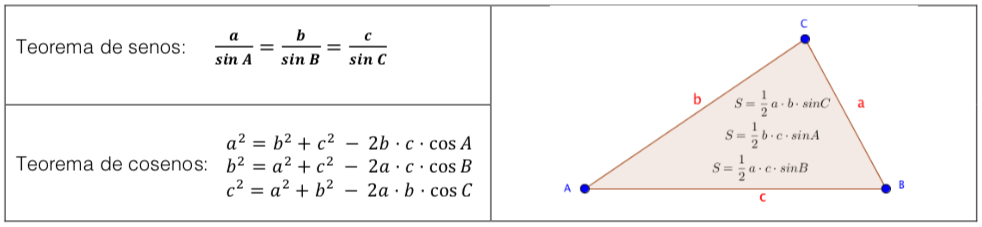
\includegraphics[width=1\textwidth]{imagenes/apendices/APENDICESIM06.png}
	\end{figure}


	\begin{figure}[H]
		\centering
		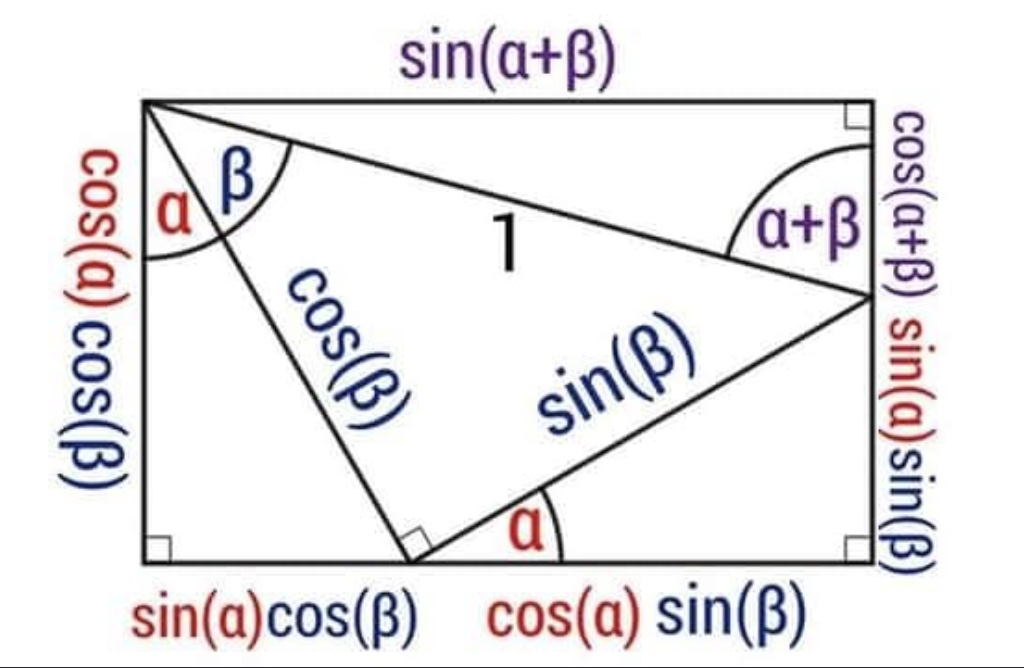
\includegraphics[width=0.6\textwidth]{imagenes/apendices/APENDICESIM10.png}
	\end{figure}



	RAZONES TRIGONOMÉTRICAS DE LA SUMA (RESTA) DE ÁNGULOS.
	
	$\sin(a \pm b)=\sin a \; cos b \pm \cos a \; \sin b \qquad \cos(a \pm b)= \cos a \; cos b \mp \sin a \; \sin b$
	
	$\tan (a\pm b) = \dfrac {\tan a \pm \tan b}{1 \mp \tan a \cdot \tan b}$
	
	RAZONES TRIGONOMÉTRICAS DEL ÁNGULO DOBLE.
	
	$\sin 2a = 2 \sin a \; cos a ; \quad \cos 2a =\cos^2 a - \sin^2 a ; \quad \tan 2a = \dfrac {2 \; \tan a}{1-\tan^2 a}$
	
	RAZONES TRIGONOMÉTRICAS DEL ÁNGULO MITAD.
	
	$\sin \dfrac a 2 = \pm \sqrt{ \dfrac {1-\cos a}{2}} ; \quad \cos \dfrac a 2 = \pm \sqrt{ \dfrac {1+\cos a}{2} ; \quad }\tan \dfrac a 2 = \pm \sqrt{\dfrac {1-\cos a}{1+\cos a}}$
	
	TRANSFORMACIÓN DE SUMAS EN PRODUCTOS:
	
	$\sin a + \sin b = 2 \sin \dfrac {a+b}{2}\cdot \cos \dfrac {a-b}{2}  ; 	\quad  \cos a + \cos b = 2 \cos \dfrac {a+b}{2}\cdot \cos \dfrac {a-b}{2}$
	
	$\sin a - \sin b = 2 \cos \dfrac {a+b}{2}\cdot \sin \dfrac {a-b}{2}  ; 	\quad  \cos a - \cos b = -2 \sin \dfrac {a+b}{2}\cdot \sin \dfrac {a-b}{2}$
	
	TRANSFORMACIÓN DE PRODUCTOS EN SUMAS.
	
	De las ecuaciones anteriores, combinándolas adecuadamente, se puede transformar el productos de un seno (o coseno ) por otro (seno o coseno).
	
	$\sin a \cdot \sin b= -\dfrac 1 2 [\cos(a+b)-\cos(a-b)]; \quad \sin a \cdot \cos b= \dfrac 1 2 [\sin(a+b)+\sin(a-b)]$
	
	$\cos a \cdot \sin b= \dfrac 1 2 [\sin(a+b)-\sin(a-b)]; \quad \cos a \cdot \cos b= \dfrac 1 2 [\cos(a+b)+\cos(a-b)]$
	
\section{Geometría analítica y vectores - 2D}
	
	\begin{figure}[H] 
		\label{araeas-volumenes}
		\centering
		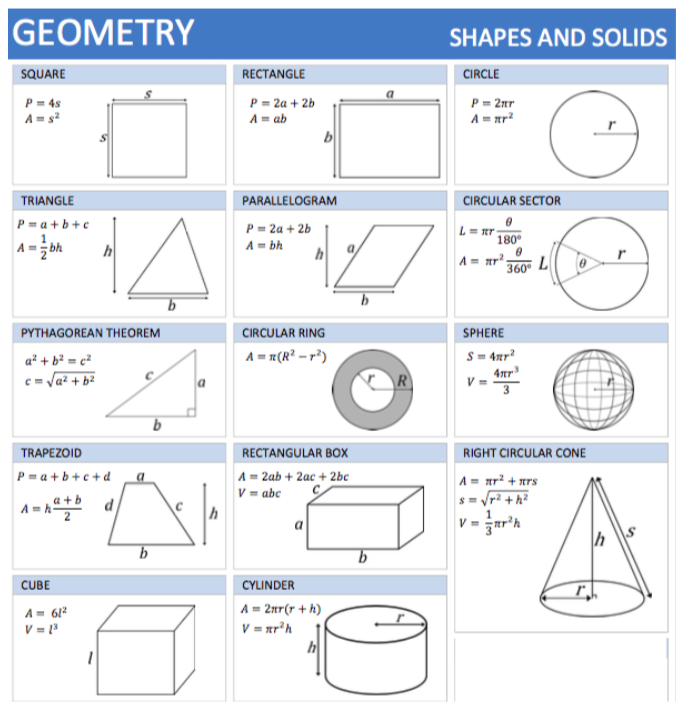
\includegraphics[width=.5\textwidth]{imagenes/apendices/APENDICESIM07.png}
		\caption{Áreas y volúmenes usuales.}
	\end{figure}

Sería conveniente recordar las áreas y volúmenes de los cuerpos más sencillos.

\begin{multicols}{2}

$d(P,Q)=|\overrightarrow{PQ}| quad $; siendo $\ \overrightarrow{PQ}=Q-P$

$\vec u \cdot \vec v = |\vec u||\vec v|\cos \theta \quad $; siendo  $ \theta= \widehat {\vec u, \vec v  }$

$\vec u \bot  \vec u \leftrightarrow \vec u \cdot \vec v =0$

$r:\; Ax+By+Cz=0 \to y=mx+n; \quad m=\tan \theta$

$r \parallel s \leftrightarrow m_r=m_s; \quad r \bot s \leftrightarrow m_r=	\dfrac {-1}{m_s} $

	\begin{figure}[H] 
		\centering
		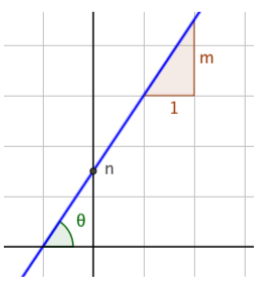
\includegraphics[width=0.3
		\textwidth]{imagenes/apendices/APENDICESIM08.png}
	\end{figure}
\end{multicols}

Circunf. centro $(a,b)$ y radio$r$: $\quad (x-a)^2+(y-b)^2=r^2 \quad $. 

Elipse semiejes $a$ y $b$: $\quad \dfrac {x^2}{a^2} + \dfrac {y^2}{b^2} = 1 	\quad $. Semidistancia focal elipse: $c$; execentricidad elipse: $0<e=\dfrac c a < 1$

\section{Análisis}

Aunque se repasan en este texto, convendría recordar lo aprendido acerca de límites, continuidad, derivadas y sus aplicaciones en el curso de primero de bachillerato.

$f$ ctna en $a$ si $\underset{x\to a}{lim}{f(x)}=f(a) \leftrightarrow \begin{cases}
 	1) & \exists f(a) \\
 	2) & \exists {lim}{f(x)} \\
 	3) & \underset{x\to a}{lim}{f(x)}=f(a)
 	\end{cases}$

Si $f$ no es continua en $a$, se dice que es discontinua: evitable, salto, asintótica.


La derivada de una función $f$ en un punto $a$ es la pendiente de la recta tangente a $f(x)$ en $x=a$ (un número real) y se define como: $f'(a)=\underset{h\to 0}{lim}{\dfrac {f(a+h)-f(a)}{h}}$. Si se define en un punto $x$ arbitrario, tenemos $f'(x)$, la función derivada.

ALGEBRA DE DERIVADAS:
		
		$(k\cdot f)'=k\cdot f' \; \quad (f\pm g)'=f' \pm g'\ ;  \quad (f\cdot g)'=f'\cdot g + f\cdot g' \ ; \quad \left({\dfrac f g}\right) '=\dfrac {f'\cdot g - f\cdot g'}{g^2}$
		
		\vspace{5mm}
		
		REGLA DE LA CADENA:  $\left({g\left (f(x) \right)}\right)' = g'\left(f(x) \right) \cdot f'(x)$
		
		\vspace{5mm}
		

		TABLA DE DERIVADAS:
		\begin{table}[hbt]
		  \centering
		   \begin{tabular}{|l|l||l|l|}
		   \hline
		   $f(x)$ & $f'(x)$ & $f(x)$ & $f'(x)$\\[5pt] \hline \hline
		   $k$ & $0$ & $x$ & $1$\\ \hline
		   $x^n$ & $n\ x^{n-1}$ & $u^n$ & $n\ u^{n-1}\ \textbf {u'}$\\ \hline
		   $\sqrt{x}$ & $\dfrac {1}{2 \sqrt{x}}$ & $\sqrt{u}$ & $\dfrac {1}{2\ \sqrt{u}}\ \textbf {u'}$\\[10pt] \hline
		   $e^x \ || \quad a^x$ & $e^x \ || \quad a^x\ \ln a$ & $e^u\ || \quad a^u$ & $e^u \ \textbf {u'}\ || \quad a^u\ \ln a\ \textbf {u'}$\\ \hline
		   
		   $\ln x\ || \quad \log_a x$ & $\dfrac {1} {x}\ || \quad \dfrac {1}{x \ \ln a}$ & $\ln u\ || \quad \log_a u$ & $\dfrac {1}{u}\ \textbf {u'}\ || \quad \dfrac {1}{u\ \ln a}\ \textbf {u'}$\\[10pt] \hline
		   $\sin x$ & $\cos x$ & $\sin u$ & $\cos u\ \textbf {u'}$ \\ \hline
		   $\cos x$ & $-\sin x$ & $\cos u$ & $-\sin u\ \textbf {u'}$ \\ \hline
		   $\tan x$ & $\dfrac {1}{\cos^2 x}=1+\tan^2 x$ & $\tan u$ & $\dfrac {1}{\cos^2 u} \ \textbf {u'} = (1+\tan^2 u)\ \textbf {u'}$\\[10pt] \hline
		   $\arcsin x$ & $\dfrac {1}{\sqrt{1-x^2}}$ & $\arcsin u$ & $\dfrac {1}{\sqrt{1-u^2}}\ \textbf {u'}$ \\[10pt] \hline
		   $\arccos x$ & $\dfrac {-1}{\sqrt{1-x^2}}$ & $\arccos u$ & $\dfrac {-1}{\sqrt{1-u^2}}\ \textbf {u'}$ \\[10pt] \hline
		   \vspace{2mm}
		   $\arctan x$ & $\dfrac {1}{1+x^2}$ & $\arctan u$ & $\dfrac {1}{1+u^2}\ \textbf {u'}$ \\ \hline
		  \end{tabular}
		\end{table}
	
	Es conveniente recordar que el signo de la primera derivada daba información sobre el crecimiento de la función, así como la presencia de máximos y mínimos relativos. El signo de la segunda derivada da la curvatura (concavidad o convexidad) de la función y la presencia de puntos de inflexión.
	
	También sería conveniente recordar los problemas de optimización hechos en primero de bachillerato, así como las funciones polinómicas y racionales representadas. 
	
	
	

\chapter{Intoducción a la lógica}
\label{ap:logica}

Este apéndice está basado en: \emph{Lógica, conjuntos, relaciones y funciones.   Álvaro Pérez Raposo.     Universidad Autónoma de San Luis Potosí; Universidad Politécnica de Madrid. Publicaciones Electrónicas Sociedad Matemática Mexicana, algunas imágenes incluidas.}

\begin{multicols}{2}
Lógica es la herramienta que usan las matemáticas para su desarrollo, es un esquema de reglas que permite deducir verdades a partir de otras verdades. El medio que lleva de las primeras verdades a las otras deducidas se llama razonamiento lógico. Lo que le importa a la lógica es saber cuándo un razonamiento es válido independientemente del contenido de las verdades que se enuncien.
	\begin{figure}[H] 
		\centering
		
\includegraphics[width=0.25
		\textwidth]{imagenes/apendices/APENDICESIM11.png}
	\end{figure}
\end{multicols}

\textbf{1. Proposiciones y variables lógicas}

Puesto que la lógica busca deducir verdades a partir de otras verdades, su materia prima son los enunciados de esas verdades. Eso es lo que llamamos \emph{proposiciones}: un enunciado que se puede juzgar como verdadero o falso.

El enunciado “  $\sqrt{2}$ es un número racional” es una proposición, pues se puede juzgar que es falso. Pero los enunciados “los números enteros son interesantes” o “los números complejos son más complicados que los reales” no son proposiciones, pues no pueden ser juzgados objetivamente.

Utilizaremos letras latinas minúsculas, especialmente $p,q,r,s,t, \cdots $ para representar proposiciones cualesquiera, pueden tener dos valores: verdadero o falso ($1$ ó $0$). Y como representan proposiciones cualesquiera, pueden tomar cualquiera de los dos. Estos símbolos ya no son proposiciones sino variables lógicas o proposicionales.

\underline{Definición}:  Una \emph{variable lógica} o variable proposicional es un símbolo que puede tomar dos valores: verdadero (representado por $1$) o falso (representado por $0$).


\small{\underline{Axioma del tercero excluido: lógica binaria}. Existen otras lógicas: lógica difusa, borrosa o heurística (una persona que mida $2$ metros es claramente una persona alta, si previamente se ha tomado el valor de persona baja y se ha establecido en $1$ metro. Se basa en reglas heurísticas de la forma SI (antecedente) ENTONCES (consecuente). SI hace muchísimo frío ENTONCES aumento drásticamente la temperatura de la calefacción. Se suele usar en redes neuronales artifiviales. SI voy a llegar un poco tarde ENTONCES aumento levemente la velocidad de mi vehículo) y lógica cuántica (cualquier valor entro $0$ y $1$, \emph{q-bits})} \normalsize{.} 

\begin{multicols}{2}
Una variable lógica p puede tomar los valores $0$ ó $1$. Si en una expresión aparecen dos variables $p$ y $q$, tenemos un total de cuatro combinaciones posibles de los valores de $p$ y $q$. Si tenemos tres variables, hay ocho posibilidades ($2^3$). Una tabla de verdad es una representación en filas y columnas de los posibles valores de las variables lógicas. En las siguientes tablas se muestran todas las posibles combinaciones de los valores 0 y 1 para dos y tres variables.
\begin{figure}[H] 
		\centering
		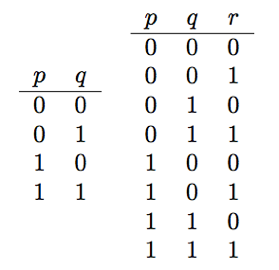
\includegraphics[width=0.4
		\textwidth]{imagenes/apendices/APENDICESIM12.png}
	\end{figure}
\end{multicols}

Es posible que una variable dependa de otras y su valor quede condicionado por ellas. En ocasiones puede ocurrir que la variable dependiente tome siempre el valor $1$ (verdadero) para cualquier situación de las variables de las que depende. O bien, que tome siempre el valor $0$ (falso). Las variables con este comportamiento reciben un nombre:

\underline{Definición}:  Se llama \emph{tautología} a la variable lógica, dependiente de otras, la cual toma el valor $1$ independientemente del valor de las variables de las que depende. Análogamente se llama \emph{contradicción} a la variable lógica cuyo valor es $0$ en cualquier situación.

\vspace{5mm}\textbf{2. Conectores de proposiciones}

Los conectores permiten construir nuevas proposiciones a partir de unas dadas. La nueva proposición es dependiente de las proposiciones con las que se construye.

Vamos a estudiar un conector monario llamado \emph{negación} el cual, a partir de una proposición, construye otra. También varios conectores binarios, que a partir de dos proposiciones dan otra: \emph{conjunción, disyunción, implicación y doble implicación}. 

Empezamos por la negación de una proposición, que es otra proposición con valor opuesto a la primera. Si la primera es cierta, su negación es falsa y viceversa.

\underline{Ejemplo}: La negación de la proposición $-5$ es un `número entero' es la proposición $-5$ `no es un número entero'.

En términos de variables lógicas, la negación de una variable es otra variable dependiente de la primera porque su valor está determinado por el de ella. 

\begin{multicols}{2}
\underline{Definición}: La negación de una proposición $p$, denotada  $\neg p$, es la proposición cuyo valor es el opuesto al de p. Se puede definir la negación mediante la siguiente tabla. En ella se indica, para cada valor de la proposición $p$, el valor que toma la proposición $\neg p$.

\begin{figure}[H] 
		\centering
		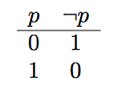
\includegraphics[width=0.25\textwidth]{imagenes/apendices/APENDICESIM13.png}
	\end{figure}
\end{multicols}


La \emph{conjunción} es un conector binario que funciona como la conjunción copulativa ``y'' del español. La conjunción de dos proposiciones es una proposición que es cierta si ambas son ciertas, y es falsa si alguna de ellas es falsa. 


\underline{Ejemplo}: `$3$ es menor que $5$ y $5$ es menor que $7$' es una proposición cierta, porque las dos proposiciones que la componen son ciertas, pero `$3$ es menor que $5$ y $8$ es menor que $4$' es falsa porque una de ellas es falsa. También es falsa '$5$ es menor que $3$ y $8$ es menor que $4$'.

\begin{multicols}{2}
\underline{Definición}. La \emph{conjunción} de dos proposiciones $p$ y  $q$, denotada por $p\;\wedge\; q$, es la proposición que \emph{sólo es cierta si ambas son ciertas}.

La definición mediante una tabla consiste ahora en ilustrar, para cada valor que pueden tomar las proposiciones $p$ y $q$, el valor que resulta en la proposición $p\wedge q$.
\begin{figure}[H] 
		\centering
		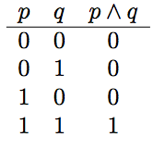
\includegraphics[width=0.3\textwidth]{imagenes/apendices/APENDICESIM14.png}
	\end{figure}
\end{multicols}

La \emph{disyunción} es el conector que opera de forma parecida a la conjunción disyuntiva ``o''  del español. La disyunción de dos proposiciones es otra proposición que es cierta si alguna de las dos originales es cierta. Es decir, basta que una de ellas sea cierta para que lo sea la disyunción. 

\underline{Ejemplo}: '$3$ es menor que $5$ o $9$ es menor que $7$' es cierta ya que una de las dos afirmaciones es cierta.

En el lenguaje habitual, la conjunción disyuntiva``o'' se suele emplear en sentido exclusivo: sólo es cierta si una de las proposiciones es cierta y la otra es falsa. Así ocurre, por ejemplo, cuando decimos `voy al cine o me quedo en casa'. Sin embargo en lógica se emplea en sentido inclusivo como se aprecia en la tabla que la define. 

\begin{multicols}{2}
\underline{Definición}: La \emph{disyunción} de dos proposiciones $p$ y $q$ , denotada $p \;  \vee \;  q$, es la proposición que \emph{sólo es falsa si ambas son falsas}.

\small{\emph{Disyunción exclusiva} :  ó $p$ ó $q$,   $p \veebar q$ (equivale a:  $(p \wedge \neg  q) \vee( \neg p \wedge q)$; su tabla de valor muestra que la disyunción exclusiva es cierta sólo cuando p ó q lo sean, pero no cuando lo sean ambas)}\normalsize{.}
\begin{figure}[H] 
		\centering
		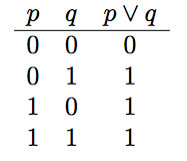
\includegraphics[width=0.3\textwidth]{imagenes/apendices/APENDICESIM15.png}
	\end{figure}
\end{multicols}

El siguiente conector que introducimos es la \emph{implicación}, que tiene gran importancia en la lógica pues es la base del razonamiento deductivo. Requiere un poco de atención para entender bien su definición formal que, al principio, no parece responder a la intuición. \emph{Cuando decimos que una proposición implica otra queremos expresar el hecho de que si la primera es cierta, entonces la segunda debe ser cierta también}.

\underline{Ejemplo}: `Si $2 < 3$, entonces $10 < 15$' es una implicación.

En el lenguaje corriente se usa la expresión \emph{“Si ...entonces ...”}. Las dos proposiciones que aparecen en la implicación se llaman antecedente y consecuente. El antecedente es la condición que, si es cierta, asegura que se cumple el consecuente. En el ejemplo anterior, $2 < 3$ es el antecedente, mientras que $10 < 15$ es el consecuente.

Para dar una definición formal debemos, como en las definiciones anteriores, decir qué valor tiene la implicación en cada caso de los posibles valores de antecedente y consecuente. Es claro que una implicación es cierta si el antecedente es cierto y el consecuente también, como ocurre en el ejemplo anterior. Si el antecedente es verdadero y el consecuente falso no se está dando la implicación y, por tanto, digo que es falsa, como en la implicación `si $2 < 3$ entonces $5 < 4$'. Quedan los dos casos en que el antecedente es falso, como la implicación `si $3 < 2$ entonces . . . '. Pero, siendo falso el antecedente, no obliga a nada al consecuente así que ambas opciones (consecuente verdadero o falso) son válidas y debo considerar que la implicación se ha cumplido (ya que no se ha incumplido).

Por todo ello definimos la implicación del siguiente modo.

\begin{multicols}{2}

\underline{Definición}: La \emph{implicación} de dos proposiciones $p$ y $q$, denotada $p \to  q$, es la proposición que \emph{sólo es falsa si $p$ es verdadera y $q$ es falsa}.

$p \to q$  es equivalente a  $\neg p \vee q$.  Comparar ambas tablas de verdad para probarlo.

\begin{figure}[H] 
		\centering
		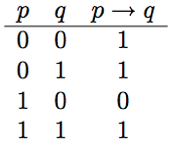
\includegraphics[width=0.3\textwidth]{imagenes/apendices/APENDICESIM16.png}
	
\end{figure}

\end{multicols}


Es fácil convencerse de que la proposición $p \to  q$ no es la misma que $q \to  p$. Basta ver la tabla de la definición anterior o analizar un ejemplo sencillo: Mientras que la implicación `si un número es real entonces su cuadrado es real' la damos por buena, al darle la vuelta obtenemos `si el cuadrado de un número es real, entonces dicho número es real', la cual no es cierta porque el número complejo $i$, que no es real, cumple $i^2 = -1\in \mathbb R$. Esta observación es suficientemente importante como para asignar nombres a cada una de estas implicaciones.

Además de la expresión `Si …. entonces ….' para la implicación , se usan también: `$p$ sólo si $q$', `$q$ si $p$', `$p$ es una condición suficiente para $q$', `$q$ es una condición necesaria para $p$', `$q$ se sigue de $p$', `$q$ a condición de $p$', `$q$ es una consecuencia lógica de $p$', `$q$ cuando $p$'.

\underline{Definición}: Dada una implicación $p \to q$, otorgamos nombres a las siguientes implicaciones: 


	\begin{figure}[H] 
		\centering
		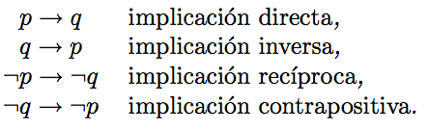
\includegraphics[width=0.7\textwidth]{imagenes/apendices/APENDICESIM17.png}
	\end{figure}

La implicación contrapositiva tambiés se llama contrarecíproca.

El último conector que introducimos es el de \emph{doble implicación o bicondicional}. Como su nombre indica, si dos proposiciones están relacionadas con el conector doble implicación, significa que una implica la otra y la otra la una. Entonces, si una de ellas es cierta, la otra debe serlo también, que es lo mismo que decir que si una es falsa la otra también.

\begin{multicols}{2}
\underline{Definición}: La \emph{doble implicación} de dos proposiciones $p$ y $q$, denotada $p \leftrightarrow q$ es la proposición que \emph{sólo es verdadera si ambas coinciden en su valor}.

 $(p \leftrightarrow q) \Leftrightarrow  (p \to  q) \wedge (q \to  p) \Leftrightarrow \cdots    \Leftrightarrow (p \wedge q) \vee ( \neg p \wedge \neg q)$

	\begin{figure}[H] 
		\centering
		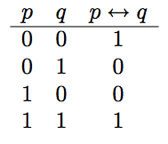
\includegraphics[width=0.3\textwidth]{imagenes/apendices/APENDICESIM18.png}
	\end{figure}
\end{multicols}

\underline{Definición}: Dos variables $p$ y $q$ son \emph{equivalentes}, y se denota $ p \Leftrightarrow q$, si $p \leftrightarrow q$ es una tautología.

Es claro que en cualquier expresión puedo sustituir una proposición por otra equivalente, y la nueva expresión que obtengo es equivalente a la original pues los valores son los mismos. De ahí que el concepto de proposiciones equivalentes sea importante y muy utilizado en lógica.

Ahora podemos enunciar un primer resultado sencillo pero muy útil en la teoría y en la práctica de la lógica. Es la relación entre las implicaciones directa, inversa, recíproca y contrapositiva (o contrarecíproca).

\underline{Teorema} : Las implicaciones directa y contrapositiva son equivalentes, y las implicaciones inversa y recíproca son equivalentes.

Simbólicamente: $\quad  p \to q \Leftrightarrow \neg q \to \neg p\; , \qquad   q \to p \Leftrightarrow \neg p \to \neg q$.

\underline{Demostración}: Probamos la primera equivalencia, pues la otra es similar. Para ello basta con elaborar una tabla con todos los casos posibles y ver que, efectivamente, en todos ellos las proposiciones directa y contrapositiva toman el mismo valor. Obsérvese que las columnas $neg p$ y $neg q$ son auxiliares en esta tabla, pues el objetivo es comparar las columnas etiquetadas como $p \to q$ y $\neg q \to \neg p$, donde se ve que la bicondicional es una tautología, pues en cualquiera de los cuatro casos el resultado es el valor $1$. Luego $p \to q \Leftrightarrow \neg q \to \neg p$.  Análogamente se Demuestra que  $q \to p \Leftrightarrow \neg p \to \neg q$. 
	
	\begin{multicols}{2}
	\begin{figure}[H] 
		\centering
		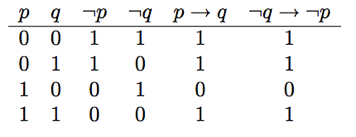
\includegraphics[width=0.5\textwidth]{imagenes/apendices/APENDICESIM19.png}
	\end{figure}
	\begin{figure}[H] 
		\centering
		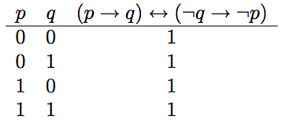
\includegraphics[width=0.5\textwidth]{imagenes/apendices/APENDICESIM20.png}
	\end{figure}
	\end{multicols}
\rightline{$\Box$}

\underline{Ejemplo}: Fijémonos en la implicación `si un número es mayor que $10$ entonces es mayor que $5$'. Es equivalente a decir `si un número no es mayor que $5$ entonces no es mayor que $10$', que es su contrapositiva.

Sin embargo no es equivalente a su implicación inversa, que es `si un número es mayor que $5$ entonces es mayor que $10$', pues cualquier número entre $5$ y $10$ muestra que no es cierta, mientras que la original sí lo es. Tampoco es equivalente a la recíproca, `si un número no es mayor que $10$ entonces no es mayor que $5$'.

Otro teorema relacionado con el concepto de equivalencia es la que dice que el conector doble implicación es equivalente a la implicación directa junto con la implicación inversa. Es la formulación precisa de lo que el símbolo $\leftrightarrow$ expresa abiertamente.

\underline{Ejercicio}: En un determinado país, todos sus habitantes cumplen la ley de `si llueve, entonces cojo el paraguas'. Analiza que ocurre cuando un determinado día llueve o no en ese país y lo que ocurre si observas a un determinado ciudadano del país con y sin paraguas.

\underline{Teorema}: La doble implicación es equivalente a la conjunción de las implicaciones directa e inversa. Es decir,   $(p \to q) \wedge (q \to  p) \Leftrightarrow (p \leftrightarrow q)$.

\underline{Demostración}: Como antes, basta elaborar las tablas de ambas proposiciones y comprobar que sus resultados son iguales para todos los valores posibles de $p$ y $q$. En este caso las dos últimas columnas deben ser iguales, mientras que las columnas $p \to q$ y $q to p$ son auxiliares. 

	\begin{figure}[H] 
		\centering
		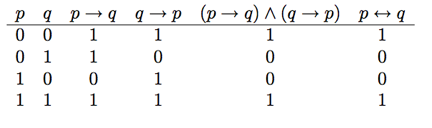
\includegraphics[width=0.7\textwidth]{imagenes/apendices/APENDICESIM21.png}
	\end{figure}

\rightline{$\Box$}

Por ser la doble implicación como dos implicaciones, se acostumbra a leer $p \leftrightarrow q$ también con la fórmula `$p$ si, y sólo si, $q$', en ocasiones abreviado como `ssi', `sii', o `syss'. Otra forma de expresar el bicondicional es decir que \emph{ $q$ es una condición necesaria y suficiente para $p$}.

La distinción entre \emph{condición necesaria} y \emph{condición suficiente} es un tema muy costoso de entender. En principio, partiendo de la denominación de cada una de estas condiciones es sencillo distinguirlas, pero en la práctica hay muchas ocasiones de confusión. Ante una condición necesaria mucha gente piensa que lo que está viendo es una condición suficiente, y viceversa. Y hasta hay ocasiones en las que teniendo una condición solamente necesaria (o solamente suficiente) se cree que en realidad es de los dos tipos, necesaria y suficiente. En general esto ocurre con las implicaciones: ``Si es cierto $A,$ entonces es cierto $B$''.

Que esto ocurra no significa ni `Si es cierto $B$, entonces es cierto $A$' ni `si no es cierto $A$$,$ entonces no es cierto B', pero en muchos casos se piensa que sí. Veamos un sencillo ejemplo: 

Está claro que ``Si llueve, entonces mi patio se moja'' (Si es cierto $A$, entonces es cierto $B$), ?`verdad? ?`Es cierto entonces que ``Si mi patio se ha mojado, entonces es que ha llovido'' (Si es cierto $B$, entonces es cierto $A$)? Claramente no, ya que mi patio puede estar mojado porque lo he hecho yo con una manguera y no por haber llovido. ?`Y es cierto que ``Si no llueve, entonces mi patio no se moja'' (Si no es cierto $A$, entonces no es cierto $B$)? Pues tampoco, por lo mismo que en el caso anterior: he podido mojarlo yo sin que haya llovido.

La primera parte de la primera frase, `Si llueve,…,'  es una condición suficiente para que mi patio se moje, pero no una condición necesaria. Es decir, es suficiente que llueva para que se moje mi patio, pero no es necesario que llueva para que ello ocurra.

\underline{Ejemplo}: La proposición ``el número entero $a$ es mayor que $b$ si, y sólo si, la diferencia $a - b$ es positiva'' significa que si $a$ es mayor que $b$, entonces tenemos la seguridad de que la diferencia $ a- b $ es un número positivo y, al revés, que si la diferencia $a - b$ es positiva, entonces sabemos que $a$ es mayor que $b$.

\underline{Ejercicio}: Sean las proposiciones $p\; $ : Está nevando;   $q\; $ : Iré a la ciudad;  $r\; $ : Tengo tiempo.  
\begin{multicols}{2}
	
a) Escribir, usando conectores lógicos, una proposición que simbolice cada una de las afirmaciones siguientes: 
\begin{itemize}
\item Si no está nevando y tengo tiempo, entonces iré a la ciudad. 
\item Iré a la ciudad sólo si tengo tiempo.
\item No está nevando.
\item Está nevando, y no iré a la ciudad.
\end{itemize} 

b) Enunciar las afirmaciones que se corresponden con cada una de las proposiciones siguientes: 
\begin{itemize}
\item $q \leftrightarrow (r \wedge  \neg p)$
\item $r \wedge q$
\item $(q \to  r) \wedge (r \to q)$ 
\item $\neg (r \vee q)$
\end{itemize} 

\end{multicols}

\textcolor{gris}{ Soluciones:}

\begin{multicols}{2}
\textcolor{gris}{(a)  Escribimos en forma simbólica las afirmaciones propuestas.}

\textcolor{gris}{$ (\neg p \wedge r) \to q \, ; \qquad   q \to  r \; ;$}

\textcolor{gris}{$  \neg p \; ; \qquad     p \wedge \neg q $}

\textcolor{gris}{(b)  Escribimos en forma de afirmaciones las proposiciones.} 

\textcolor{gris}{-- Iré a la ciudad si, y sólo si tengo tiempo y no está nevando.}

\textcolor{gris}{-- Tengo tiempo e iré a la ciudad.}       

\textcolor{gris}{-- Iré a la ciudad si y sólo si tengo tiempo.}       

\textcolor{gris}{--Ni tengo tiempo, ni iré a la ciudad.} 
\end{multicols}

\underline{Ejercicio}:  Sean $p$ `tengo un loro' y $q$ `tengo un gato', escribir en lenguaje corriente y luego simplificar:
$\displaystyle \neg \left( \dfrac {}{} \neg p \; \vee \neg (\neg q) \right) \; \wedge \; \neg (\neg p) $



\textcolor{gris}{Solución:  Simplifiquemos la expresión dada, 
$\; \displaystyle \neg \left( \dfrac {}{} \neg p \; \vee \neg (\neg q) \right) \; \wedge \; \neg (\neg p) \equiv (p \wedge \neg q) \wedge p \equiv p \wedge (\neg q \wedge p ) \equiv p \wedge (p \wedge \neg q) \equiv (p \wedge p) \wedge \neg q \equiv p \wedge \neg q\; $.  
Luego es equivalente a afirmar: ``tengo un loro y no tengo un gato''.} 

\underline{Ejercicio}:  Pruebe que:
$\; a)\; \;  \; \left[ \; (a \to b) \wedge (b \to c) \to (a \to c \; \right]  ; \quad    b)\; \; a \to b \to  \left[ \; (c \vee a) \to (c \vee b) \; \right]   $

\textcolor{gris}{Solución: construye las tablas de verdad, ambas son tautologías.}

\underline{Ejercicio}:   
Siendo $p$ y $q$ proposiciones cualesquiera, la proposición, $(p \to q)  \leftrightarrow \left[ \, (p \vee q) \leftrightarrow q  \; \right] $:  a) ?`Es siempre verdadera?;  \hspace{3mm} b) ?`Es verdadera si y sólo si p lo es?; \hspace{3mm} c) ?`Es verdadera si y sólo si q es falsa?; \hspace{3mm} d) ?`Es verdadera si y sólo si p y q lo son?

\textcolor{gris}{Solución: construyendo su tabla de verdad se ve que se trata de una tautología, es decir, es siempre verdadera.}

\vspace{5mm}\textbf{3. Leyes del álgebra proposicional (Boole)}

Los conectores entre proposiciones (negación, conjunción, disyunción, etc.) se pueden ver, desde un punto de vista algebraico, como operaciones definidas en el conjunto de las proposiciones. Se toma una proposición (en el caso de la negación, operador monario) o dos proposiciones (en los otros casos, operadores binarios) y se operan, obteniendo como resultado otra proposición.

Bajo este punto de vista resulta imperativo estudiar algunas propiedades algebraicas de estas operaciones como son la aplicación reiterada, asociatividad, conmutatividad, existencia de elemento neutro, etc.

Como primer paso veamos que los conectores de implicación y doble implicación se pueden escribir en términos de la negación, conjunción y disyunción solamente. Entonces bastará con estudiar las propiedades algebraicas de estas tres operaciones. 

\underline{Teorema}. La implicación de dos proposiciones es equivalente a la disyunción de la negación de la primera con la segunda:
   $\; \; p \to q \; \Leftrightarrow \; \neg p \wedge q$

Demostración.
	\begin{figure}[H] 
		\centering
		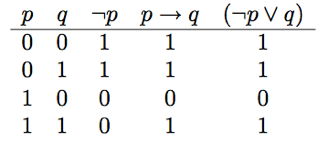
\includegraphics[width=0.5\textwidth]{imagenes/apendices/APENDICESIM22.png}
	\end{figure}

\rightline{$\Box$}	


Por tanto, en cualquier expresión podemos sustituir $p \to q$ por $\neg p \vee q$ y viceversa.

Puesto que ya vimos en un teorema anterior, la doble implicación  equivale a la implicación directa y la inversa, entonces, la doble implicación se puede expresar sólo con negación, conjunción y disyunción.

\textbf{Propiedades de la negación}

Debido a que la negación es una operación monaria, la única propiedad que en este caso puede analizarse es la aplicación reiterada. El resultado es muy evidente por estar trabajando con proposiciones que sólo pueden tomar dos valores (lógica binaria). La negación es cambiar el valor de una proposición, y como sólo hay dos posibilidades, si se cambia dos veces regresamos al valor original.

\underline{Teorema}: La negación de la negación es equivalente a la proposición original. Es decir, 

\centerline{$\neg (\neg p) \Leftrightarrow p$}

\underline{Demostración}. 
	\begin{figure}[H] 
		\centering
		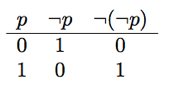
\includegraphics[width=0.3\textwidth]{imagenes/apendices/APENDICESIM23.png}
	\end{figure}
\rightline{$\Box$}


\underline{Ejemplo}: Es interesante constatar que la propiedad de la doble negación no se respeta en muchas expresiones del lenguaje coloquial. Por ejemplo, puesto que “nadie” es la negación de “alguien”, la proposición “no hay nadie” es la doble negación de “hay alguien” y, por tanto, deberían ser equivalentes. Sin embargo normalmente se usan como opuestas. 

\textbf{Propiedades de la conjunción}

La conjunción es una operación binaria y en ella sí procede estudiar más propiedades. La idempotencia, por ejemplo, da el resultado de operar una proposición consigo misma. La asociatividad nos indica cómo podemos efectuar la conjunción de tres proposiciones. La conmutatividad muestra que el orden de las proposiciones en una conjunción es irrelevante. Existe un elemento neutro (la proposición con valor $1$ que denotaremos simplemente como $1$) que al operarlo con cualquier proposición da como resultado la misma proposición. Existe también un elemento dominante (la proposición con valor $0$, que denotaremos simplemente como $0$) que al operarlo con cualquier proposición arroja el resultado $0$.

\underline{Teorema}: La conjunción de proposiciones satisface las propiedades de idempotencia, asociatividad, conmutatividad, existencia de un elemento neutro y de un elemento dominante o absorvente.

Simbólicamente, si $p$, $q$ y $r$ son proposiciones cualesquiera se cumple:

\begin{itemize}
\item 1. Idempotencia:  $\quad p \wedge p \Leftrightarrow p$ 
\item 2. Asociatividad: $\quad (p \wedge q) \wedge r \Leftrightarrow p \wedge (q \wedge r)$  
\item 3. Conmutatividad: $\quad p \wedge q \Leftrightarrow q \wedge p$  
\item 4. Elemento neutro ($1$):  $\quad p \wedge 1 \Leftrightarrow p  $
\item 5. Absorción  ($0$):  $\quad p \wedge 0 \Leftrightarrow 0$ 
\end{itemize}

\underline{Demostración}: La idempotencia está demostrada en la misma definición de la operación $\wedge$ , pues en ella se aprecia que $1 \wedge 1 = 1$ y $0 \wedge 0 = 0$. En la tabla también se prueba la conmutatividad. Asimismo se ve que $1$ sirve como neutro y que $0$ operado con cualquier otro da como resultado el valor  $0$ . Entonces sólo resta probar la propiedad asociativa. Construimos una tabla de las proposiciones $(p \wedge q ) \wedge r$ y $p \wedge (q \wedge r)$.
La igualdad de las dos últimas columnas prueba que ambas proposiciones son equivalentes. 

\begin{figure}[H] 
		\centering
		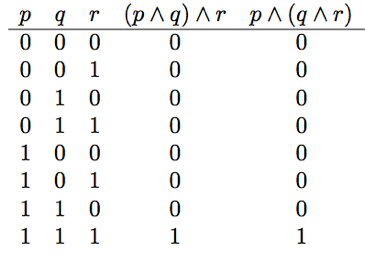
\includegraphics[width=0.5\textwidth]{imagenes/apendices/APENDICESIM24.png}
	\end{figure}
\rightline{$\Box$}

La presencia de la propiedad asociativa permite definir el símbolo $p \wedge q \wedge r$, sin paréntesis, como $(p \wedge q) \wedge r$ o bien $p \wedge (q \wedge r)$, puesto que son iguales. El resultado en ambos casos es que $p \wedge q \wedge r$ sólo es cierta si las tres proposiciones $p$, $q$ y $r$ son ciertas. Generalizando esta idea definimos la conjunción de las variables $p_1, p_2, \cdots, p_n$, denotada $p_1 \wedge p_2 \wedge \cdots \wedge p_n$, como la variable que sólo es cierta si todas las variables $p_1, p_2, \cdots , p_n$ son ciertas. 

\textbf{Propiedades de la disyunción}

El estudio de la disyunción sigue los mismos pasos que el de la conjunción pues las propiedades que satisfacen son las mismas. La única diferencia es que los papeles de $1$ y $0$, como elementos neutro y absorvente respectivamente, se invierten ahora.

\underline{Teorema}:   si $p$, $q$ y $r$ son proposiciones cualesquiera, se cumple:
\begin{itemize}
\item 1. Idempotencia:   $\quad p \vee p \Leftrightarrow p$
\item 2. Asociatividad:   $\quad (p \vee q) \vee r \Leftrightarrow p \vee ( q \vee r)$
\item 3. Conmutatividad:   $ \quad p \vee q \Leftrightarrow q \vee p$
\item 4. Elemento neutro ($0$):   $\quad p \vee 0 \Leftrightarrow p$ 
\item 5. Dominación ($1$):   $\quad p \vee 1 \Leftrightarrow 1$
\end{itemize}

La demostración se deja como ejercicio.

Como en el caso de la conjunción, $p \vee q \vee r$ es cierta si alguna de las tres es cierta, o bien, es falsa sólo si todas son falsas. Generalizando esta idea definimos la disyunción de las variables $p_1, p_2, \cdots , p_n,$ denotada $p_1 \vee p_2 \vee \cdots \vee  p_n$, como la variable que sólo es falsa si todas las variables p1, $p_1, p_2, \cdots , p_n,$  son falsas.

\textbf{Propiedades de las operaciones combinadas}

Ahora estudiamos algunas propiedades que surgen al considerar expresiones con dos o las tres operaciones combinadas.

\underline{Teorema}: Las siguientes relaciones son válidas para cualesquiera proposiciones p, q, r:

\begin{itemize}	
\item Complementariedad de la negación: 

$\qquad p \wedge \neg p \Leftrightarrow 0; \quad p \vee \neg p \Leftrightarrow 1 $ 

\item Leyes distributivas: 

$\qquad p \wedge (q \vee r) \Leftrightarrow (p \wedge q ) \vee (p \wedge r ) \; ;$
$\quad p \vee (q \wedge r) \Leftrightarrow (p \vee q ) \wedge (p \vee r )$

\item Absorción: 

$\qquad p \wedge (p \vee q) \Leftrightarrow p\; ; \quad p \vee (p \wedge q) \Leftrightarrow p$

\item Leyes de De Morgan: 
 
$\qquad \neg (p \wedge q ) \Leftrightarrow \neq p \vee \neg q\; ; \neg (p \vee q) \Leftrightarrow \neg p \wedge \neg q $

\end{itemize}

\underline{Demostración}: Ejercicio. Ver las siguientes tablas de verdad. 

\begin{figure}[H] 
		\centering
		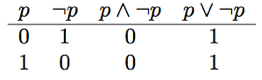
\includegraphics[width=0.3\textwidth]{imagenes/apendices/APENDICESIM25.png}
	\end{figure}
\begin{figure}[H] 
		\centering
		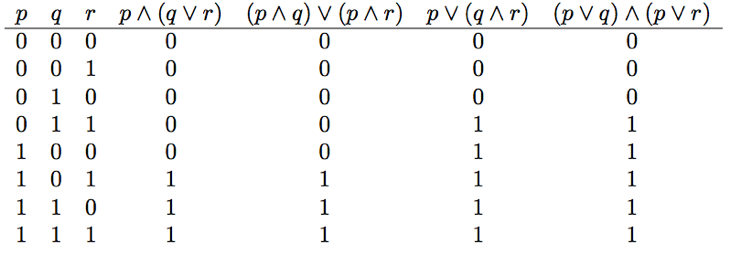
\includegraphics[width=0.9\textwidth]{imagenes/apendices/APENDICESIM26.png}
	\end{figure}
\begin{figure}[H] 
		\centering
		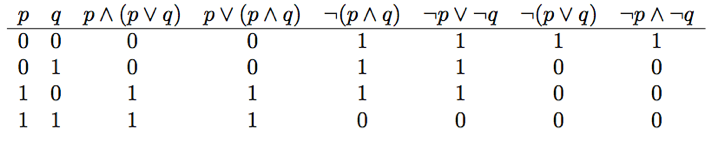
\includegraphics[width=0.9\textwidth]{imagenes/apendices/APENDICESIM27.png}
	\end{figure}
\rightline{$\Box$}


Las leyes demostradas permiten hacer manipulaciones algebraicas con las proposiciones y probar algunos resultados sin necesidad de recurrir a las tablas. Veamos unos ejemplos.

\underline{Ejemplo}: Simplificación de una proposición mediante manipulaciones algebraicas. Cada proposición es equivalente a la anterior por la ley algebraica que se indica a su lado.

\begin{figure}[H] 
		\centering
		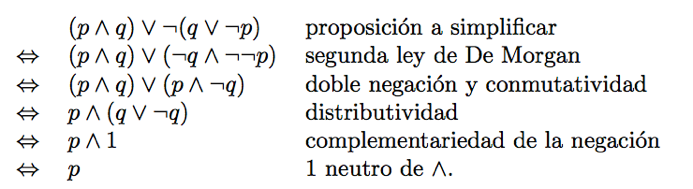
\includegraphics[width=0.8\textwidth]{imagenes/apendices/APENDICESIM28.png}
	\end{figure}

\underline{Ejemplo}: Prueba algebraica de la ley de absorción (suponiendo probadas las leyes algebraicas anteriores). Partiendo de la proposición $p \wedge (p \vee q)$, mediante pasos algebraicos llegamos a que es equivalente a la proposición $p$.

\begin{figure}[H] 
		\centering
		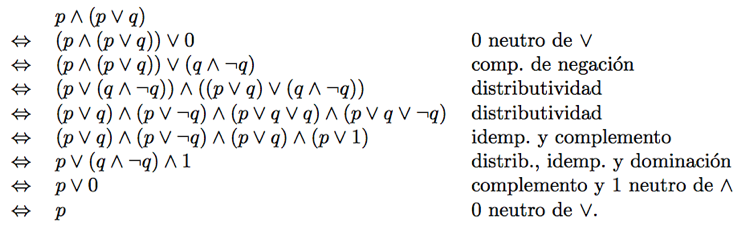
\includegraphics[width=0.9\textwidth]{imagenes/apendices/APENDICESIM29.png}
	\end{figure}


\underline{Ejercicio}:  Simplifique las siguientes expresiones:

$a)\;  (p \vee q) \to (\neg p \wedge q);\quad    b)\; [(p \wedge q) \vee r ]\wedge \neg q ;\quad   c)\; [(p \to q) \to p] \to (p \vee q) $

\textcolor{gris}{\underline{Solución}:}

\begin{figure}[H] 
		\centering
		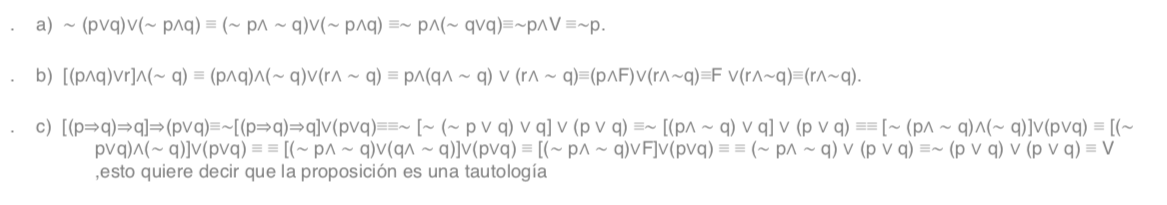
\includegraphics[width=1.1\textwidth]{imagenes/apendices/APENDICESIM33.png}
	\end{figure} 

\underline{Ejercicio}:  Se sabe que:  Si Pedro no es alumno de la U. V. o Juan es alumno de la U. V., entonces Juan es alumno de la U. P. C.  Si Pedro es alumno de la U. V. y Juan no es alumno de la U. P. C., entonces Juan es alumno de la U. V.  Se desea saber en que universidad estudia Juan.

\textcolor{gris}{\underline{Solución}:  Sean $p$: Pedro es alumno de la U.V.,  $q$: Juan es alumno de la U.P.V. y  $r$: Juan es alumno de la U.V.}

\begin{figure}[H] 
		\centering
		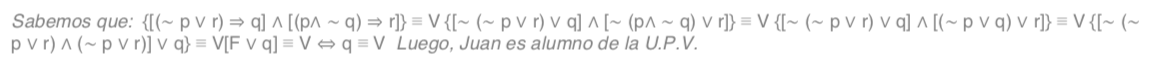
\includegraphics[width=1.1\textwidth]{imagenes/apendices/APENDICESIM34.png}
	\end{figure} 

\vspace{5mm}\textbf{4. Cuantificadores}

En esta sección introducimos los enunciados abiertos y, tras ellos, los cuantificadores. Son elementos muy habituales en la formulación de definiciones y resultados en matemáticas en expresiones de la forma “para todo número entero ...” o “existe una función tal que ...”.

\underline{Definición}: Llamamos abierto a un enunciado que contiene variables que toman valores en un conjunto dado, llamado universo, de forma que para cada valor que tomen las variables, el enunciado se convierte en una proposición.

\underline{Ejemplo}: Si la variable $x$ toma valores en el universo de los dígitos (los números $0,1,2,3,4,5,6,7,8,9$), el enunciado “el número $x$ es mayor que $5$” es abierto.

Un enunciado abierto no es una proposición por sí mismo, sino que se convierte en una cuando las variables toman un valor. En el ejemplo anterior, el enunciado puede ser verdadero o falso según los valores que tome la variable.

Puesto que las proposiciones las representamos por letras $p, q, r, \cdots,$ los enunciados abiertos los representamos por símbolos como $p(x), q(x, y), r(x, y, z), \cdots$ donde $x, y, z$ son las variables que contiene el enunciado.

Los cuantificadores son unos prefijos que, antepuestos a enunciados abiertos, los convierten en proposiciones. Utilizaremos dos: el \emph{cuantificador universal} y el \emph{cuantificador existencial}. El primero se simboliza por $\forall$, y se suele leer “para todo”. Indica que el enunciado que le sigue debe ser cierto para todos los posibles valores de la variable. El segundo se simboliza por $\exists$, y se lee “existe algún”. Indica que el enunciado que sigue es cierto para, al menos, uno de los valores que puede tomar la variable.

Tomamos su propiedad de convertir enunciados abiertos en proposiciones como base para dar una definición.

\underline{Definición}: Si $p(x)$ es un enunciado abierto que depende de la variable $x$, la cual toma valores en un conjunto universo dado, definimos el símbolo $\forall x, p(x)$ como la proposición que es cierta sólo si el enunciado abierto es verdadero para todos los valores que la variable puede tomar en su universo.

Asimismo definimos el símbolo $\exists x, p(x)$ como la proposición que es cierta si el enunciado abierto es verdadero para algún valor de los que la variable toma en su universo.

La proposición $\forall x , p(x)$ no es en realidad otra cosa que una conjunción, mientras que $\exists x, p(x)$ se trata de una disyunción como se aprecia en el siguiente ejemplo.

\underline{Ejemplo}: Continuando el ejemplo anterior, donde la variable $x$ toma valores en los dígitos, es decir, puede valer $0, 1, 2, ..., 9$, llamamos $p(x)$ a la proposición “$x$ es mayor que $5$”. Entonces, la proposición $\forall x , p(x)$ equivale a $p(0) \wedge p(1) \wedge \cdots \wedge   p(9)$ y, claro está, es falsa. Por otro lado, la proposición $\exists x , p(x)$ equivale a $p(0) \wedge p(1) \wedge \cdots \wedge p(9)$ y, sí, es cierta.

Para usar cuantificadores basta recordar que un cuantificador junto a un enunciado abierto es una proposición y, a partir de ahí, se maneja como cualquier otra proposición. Sin embargo hay algunas reglas que simplifican el uso de proposiciones que contienen cuantificadores. En concreto analizaremos dos de ellas: la negación de proposiciones con cuantificadores y la combinación de cuantificadores.

Una proposición que comienza con el cuantificador universal necesita que el enunciado abierto sea cierto para todos los valores de la variable, por tanto basta con que en un valor sea falso para que toda la proposición sea falsa. Por ello, la negación con un cuantificador universal nos lleva a un cuantificador existencial y viceversa. Si recordamos que $\forall x , p(x)$ es una conjunción y $\exists x , p(x)$ es una disyunción, esto no es otra cosa que las leyes de De Morgan vistas en un teorema anterior. El resultado preciso se recoge en el siguiente teorema.

\underline{Teorema}: Si $p(x)$ es un enunciado abierto, con $x$ una variable, entonces se cumplen las equivalencias

$\qquad \neg (\;\forall x , p(x) \; ) \Leftrightarrow \exists x , \neg p(x)\; \qquad$
$\qquad \neg (\;\exists x , p(x) \; ) \Leftrightarrow \forall  x , \neg p(x)$


\underline{Demostración}: Como se ha dicho, se trata de las leyes de De Morgan. Razonemos una de ellas como muestra. La negación de la proposición $\forall x, p(x)$ es cierta si el enunciado $p(x)$ no se cumple en algún valor de la variable. Pero eso es precisamente lo que dice la proposición $\exists x, \neg p(x)$
\rightline{$\Box$}

Si un enunciado abierto contiene varias variables, se necesita un cuantificador para cada una. Así, si $p(x,y)$ es un enunciado abierto con las variables $x$ e $y$, entonces $ \forall x , p(x,y),\;  \exists x , p(x,y)$ son enunciados abiertos con una variable $y$. Pero $\forall x, \; \forall y, \; p(x,y); $

\hspace{-7mm} $ \forall x, \; \exists y, \; p(x,y)$ son proposiciones. La combinación de varios cuantificadores tiene algunas reglas que permiten simplificar su escritura, pero requiere atención pues no todos los casos son simplificables.

Las primera y segunda reglas nos dicen que combinar cuantificadores universales y combinar cuantificadores existenciales es conmutativo.

\underline{Teorema}:  Si $p(x, y)$ es un enunciado abierto que depende de dos variables, $x,\; y$, se cumplen las siguientes equivalencias entre proposiciones.

$\qquad \forall x, \; \forall y, \; p(x,y) \Leftrightarrow
\forall y, \; \forall x, \; p(x,y) \qquad$
$\qquad \exists x, \; \exists y, \; p(x,y) \Leftrightarrow \exists y, \; \exists x, \; p(x,y)$


\underline{Demostración}: La proposición $\forall x, \; \forall y, \; p(x,y)$ sólo es verdadera si dado cualquier $x$, puedo elegir cualquier $y$ y obtengo que $p(x, y)$ es verdadero. Pero en tal caso el valor de $y$ elegido es independiente de $x$, y puedo escogerlo primero $y$ y luego a $x$. Entonces, dado cualquier $y$, puedo elegir cualquier $x$ y tendré $p(x, y)$ verdadero, lo cual es la proposición $forall y, \; \forall x, \; p(x,y)$. Con esto se ha probado que cuando la primera es cierta, la segunda también. El mismo razonamiento pero a la inversa muestra que cuando la segunda es cierta la primera también. En total ambas tienen siempre el mismo valor y, por tanto, son equivalentes.

Análogamente la proposición $\exists x, \; \exists y, \; p(x,y)$ afirma que existe algún x de modo que puedo encontrar una y tal que $p(x, y)$ es verdadero. Puedo tomar los valores en orden inverso: escoger primero el valor de $y$ encontrado antes, luego el de $x$ y tendré $p(x, y)$ verdadero. Hemos probado, pues, que si $\exists x, \; \exists y, \; p(x,y)$ es cierta, entonces $\exists y, \; \exists x, \; p(x,y)$ también lo es. El mismo razonamiento se aplica a la inversa y llegamos a que ambas son equivalentes. 

\rightline{$\Box$}

Gracias a este resultado podemos escribir sin ambigüedad $\forall x, y$  ó   $\forall y, x$ en lugar de $\forall x, \forall y$, así como $\exists x, y$ ó $\exists y, x$ en lugar de $\exists x , \exists y$, y el orden de las variables $x$ e $y$ es irrelevante.

Sin embargo hay que tener cuidado pues el orden sí es importante cuando se combinan cuantificadores de ambos tipos, como muestra el siguiente ejemplo.

\underline{Ejemplo}: Consideremos el enunciado abierto “$x \neq y$” donde $x$, $y$ toman valores en el conjunto de los números enteros. Entonces la proposición $\forall x, \exists y, x \neq y$ afirma que un número entero cualquiera, $x$, existe al menos un número, $y$, que es distinto de él, lo cual es cierto. Sin embargo, la proposición $\exists x, \forall y ,x \neq y$ afirma que existe al menos un número entero, $x$, tal que cualquier número entero, $y$, es distinto de él, lo cual es falso.

Para terminar esta sección definimos el \emph{cuantificador de existencia y unicidad}, simbolizado $\exists\, !$. Como su nombre indica este símbolo contiene dos afirmaciones: primero, la existencia de un elemento que cumple el enunciado; segundo, que dicho elemento es el único que lo cumple. La forma de enunciar la unicidad es diciendo que si hay dos elementos que cumplen la propiedad, entonces son iguales. Todo esto se reúne en la siguiente definición.

\underline{Definición} Si $p(x)$ es un enunciado abierto, el símbolo $\exists \, !\; x , p(x)$ es la proposición definida por $(\; \exists x , p(x)\; ) \wedge \forall a, b, (\; p(a)\wedge p(b) \to a=b\; )   $.

\underline{Ejemplo}; La proposición $\exists \, !x , x2 = x$, donde $x$ 

toma valores en los enteros, significa que existe un entero, y sólo uno, que verifica que elevado al cuadrado se queda igual. Se trata de una proposición falsa puesto que, aunque cumple la existencia ($x = 1$ lo verifica), no cumple la unicidad (porque $x = 0$ también lo verifica).

\underline{Ejemplo}: La proposición 

$\exists \,!x, \forall y,\;  x + y = y$, 

donde tanto $x$ como $y$ toman valores enteros, enuncia que hay un número entero, y sólo uno, que sumado a cualquier otro lo deja igual; es decir, un elemento neutro de la suma. Esta proposición sí es cierta, lo cual se demuestra en dos pasos. Primero, la existencia: el $0$ cumple lo dicho. Segundo, la unicidad: hay que probar que si hay dos elementos neutros, llamémoslos $x_1$ y $x_2$, entonces son iguales. Ahora bien, puesto que $x_1$ es neutro, sumado con $x_2$ resulta $x_1 +x_2 = x_2$. Por la misma razón, pues $x_2$ también es neutro, tenemos $x_2 + x_1 = x_1$. Por último, por la propiedad conmutativa de la suma sabemos que $x_1 + x_2 = x_2 + x_1$, de donde concluimos que $x_1 = x_2$.

\underline{Ejercicio}:  Negar los siguientes enunciados:

$a)\;  \exists y, p(y) \to \forall x, (\,\neg q(x)\,); $
$\quad    b)\;  \exists x , (\, \neg p(x)\, ) \to \forall x, q(x); $
$\quad   c)\;  \exists x\; \forall y\, p(x,y) \to q(x,y))$

Solución:

 \begin{figure}[H] 
		\centering
		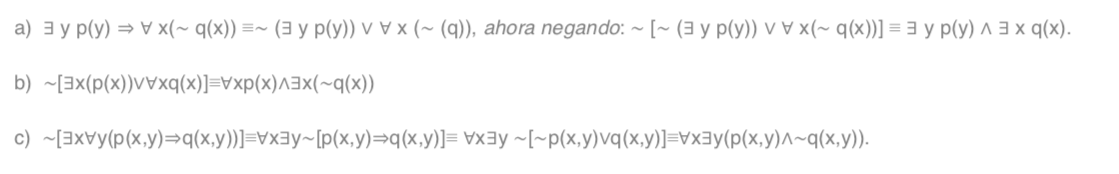
\includegraphics[width=1.1\textwidth]{imagenes/apendices/APENDICESIM35.png}
	\end{figure} 

\underline{}Ejercicio:  Negar la siguiente expresión:
$(\forall \varepsilon >0)\; (\exists \delta >0)\; (0<|x-x_0|<\delta) \to |f(x)-f(x_0)|<\varepsilon   $

Solución:
 \begin{figure}[H] 
		\centering
		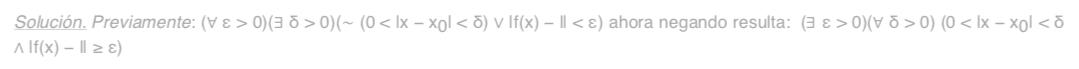
\includegraphics[width=1.1\textwidth]{imagenes/apendices/APENDICESIM36.png}
	\end{figure}


\vspace{5mm}\textbf{5. El razonamiento lógico}

Abordamos finalmente el objetivo de la lógica: obtener proposiciones verdaderas a partir de otras proposiciones verdaderas ya conocidas. Esta deducción se efectúa mediante lo que se llama un razonamiento lógico. 

Lo que se pretende con un razonamiento lógico es deducir una proposición verdadera nueva a partir de otras proposiciones verdaderas ya conocidas. Analicemos esta idea, empezando por nombrar sus elementos. Las proposiciones que son conocidas se llaman \emph{hipótesis} o premisas. La proposición que se deduce es la \emph{tesis}, resultado o consecuencia. El hecho de que las premisas nos lleven a deducir la consecuencia se puede expresar por medio de una implicación: si las premisas son ciertas, entonces la consecuencia debe ser cierta. Si $p_1, p_2, \cdots , p_n$  son las premisas y $q$ es la consecuencia, quiero expresar la idea de que si todas las premisas son ciertas, entonces la consecuencia es cierta. Es decir$ p1 \wedge p2 \wedge \cdots \wedge pn \to  q$.

Ahora, la idea clave: nos interesa el razonamiento lógico independientemente del contenido de las proposiciones. Si es cierto que de las premisas  $p_1, p_2, \cdots , p_n$  se sigue necesariamente la consecuencia $q$, entonces la expresión $ p1 \wedge p2 \wedge \cdots \wedge pn \to  q$ debe ser siempre verdadera. Esta idea se recoge elegantemente en la siguiente definición.

\underline{Definición} Una proposición de la forma $ p1 \wedge p2 \wedge \cdots \wedge pn \to  q$  es un razonamiento lógico si es una tautología. Entonces el razonamiento se denota $ p1 \wedge p2 \wedge \cdots \wedge pn \Rightarrow  q$  las proposiciones $p_1, p_2, \cdots , p_n$  se llaman premisas y la proposición $q$ consecuencia.

\underline{Ejemplo}: Consideremos las proposiciones “si un número entero no es cero, entonces su valor absoluto es positivo” y “$-4$ no es cero”. Puedo deducir que el valor absoluto de $-4$ es un número positivo. Pero la deducción no depende de que estemos hablando acerca del valor absoluto de números enteros, sino de su estructura lógica. Las premisas son $p \to  q$ (“si un número entero no es cero, entonces su valor absoluto es positivo”) y p (“un número entero, $-4$, no es cero”), es decir, $(p \to  q) \wedge p$, y la consecuencia es $q$ (“su valor absoluto, $| - 4|$, es positivo”). El razonamiento ha sido $(p \to  q) \wedge p \Rightarrow q$ y es válido sean quienes sean $p$ y $q$. Por ello tiene nombre propio: \emph{modus ponendo ponens} (del latín, que se puede traducir como el razonamiento que afirmando $p$ (ponendo) afirma $q$ (ponens )).

Veamos otros dos ejemplos de razonamiento lógico.

\underline{Ejemplo}: Con la misma implicación de antes “si un número entero no es cero, entonces su valor absoluto es positivo” y además con la proposición “el valor absoluto del número $a$ no es positivo”, puedo deducir que “el número $a$ es cero”.

El razonamiento en este caso ha sido $(p \to q) \wedge \neg q \Rightarrow  \neg p$, y se llama \emph{modus tollendo tollens} (el razonamiento que negando $q$ (tollendo) niega $p$ (tollens).

\underline{Ejemplo}: Un último ejemplo con estas proposiciones. Si tengo las dos implicaciones “si un número entero no es cero, entonces su valor absoluto es positivo” y “si un número entero $a$ es positivo, entonces $a$ es mayor que su opuesto, $-a$”, puedo deducir que “si un número entero $a$ no es cero, entonces $|a| > -|a|$”.

Este razonamiento, cuya estructura es $(p \to  q) \wedge (q to r) \Rightarrow (p to r)$, se llama \emph{silogismo}.



La pregunta ahora es, dado una expresión de la forma $ p1 \wedge p2 \wedge \cdots \wedge pn \to  q$, ?`cómo saber si es un razonamiento lógico o no? Las dos formas de probar que es un razonamiento lógico son: Primera, demostrar directamente que dicha proposición es una tautología, por ejemplo mediante una tabla. Es útil para razonamientos sencillos, cuyas tablas no sean grandes. Segunda, descomponer el razonamiento en razonamientos más simples ya conocidos. Es decir, partiendo de las premisas y aplicando razonamientos simples conocidos ir deduciendo nuevas proposiciones ciertas hasta llegar a la que se enunciaba como consecuencia. Este segundo es el método habitual de probar la validez de razonamientos lógicos complejos.

Para poder utilizar cadenas de razonamientos simples en la prueba de un razonamiento complicado necesitamos tener algunos razonamientos ya demostrados de forma directa. En el siguiente teorema se exponen algunos de estos razonamientos que son muy habituales y, prácticamente, podríamos decir que responden en gran medida al sentido común: se llaman \emph{reglas de inferencia} y tienen nombres propios.

 	\begin{figure}[H] 
		\centering
		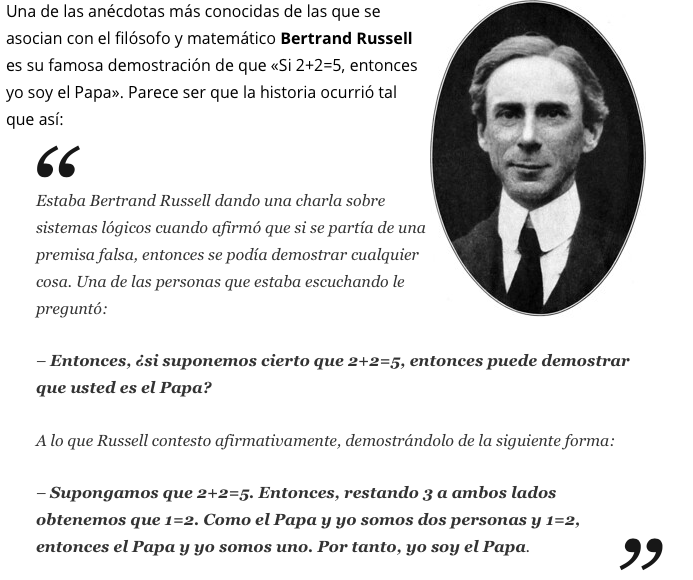
\includegraphics[width=.85\textwidth]{imagenes/apendices/APENDICESIM37.png}
		\caption{Captura de pantalla tomada del blog gaussianos.com}
	\end{figure}

\underline{Teorema}: Para proposiciones cualesquiera $p, q, r, s$ los siguientes son razonamientos lógicos:

\begin{itemize}
\item 1. Modus ponendo ponens:    	$\qquad (p \to  q) \wedge p   \Rightarrow    q$ 

\item 2. Modus tollendo tollens:     $\qquad  (p \to  q) \wedge \neg q  \Rightarrow  \neg p$ 

\item 3. Silogismo:     $\qquad   (p\to q) \wedge (q\to r)  \Rightarrow   p\to r$ 

\item 4. Demostración por contradicción:   $\qquad  (\neg p \to  0)  \Rightarrow  p$ 

\item 5. Demostración por casos:   $\qquad (p\to r) \wedge (q \to r)    \Rightarrow   (p \vee q) \to r$ 

\item 6. Silogismo disyuntivo:  $\qquad (p \vee q) \wedge (\neg p)   \Rightarrow   q$ 

\item 7. Conjunción: $\qquad (p) \wedge (q)   \Rightarrow  (p \wedge q)$ 

\item 8. Simplificación conjuntiva: $( p \wedge q)  \Rightarrow p$ 

\item 9. Amplificación disyuntiva: $ p \Rightarrow  (p \vee q)$ 

\item 10.   Especificación universal: $\qquad \forall x, p(x) \Rightarrow p(a)$,  con $a$ un elemento cualquiera del universo de $x$. 

\item 11.   Generalización universal: $\qquad (\,p(a) \wedge (\, a \text{ es arbitrario })\,) \Rightarrow \forall x , p(x)$ 

\item 12.   Especificación existencial: $\qquad \exists x , p(x) \Rightarrow p(a)$, con $a$ el elemento al que se refiere la existencia. 
\end{itemize}

\underline{Demostración}: Todas estas reglas de inferencia se pueden probar elaborando la tabla correspondiente, pero también mediante manipulaciones algebraicas. En cualquier caso son todas muy similares, por lo cual expondremos la prueba de tres de ellas con todo detalle, a modo de muestra, dejando el resto como ejercicio.

Prueba del \emph{modus ponendo ponens} mediante una tabla. Para probar ((p ? q)?p) ? q debemos probar que $(p \to  q) \wedge p) \Rightarrow q$ es una tautología. 

\begin{figure}[H] 
		\centering
		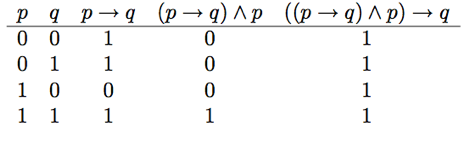
\includegraphics[width=.85\textwidth]{imagenes/apendices/APENDICESIM30.png}
	\end{figure}

La última columna muestra que, efectivamente, la implicación es una tautología y por tanto el razonamiento es válido.

Prueba del \emph{razonamiento por contradicción} mediante manipulaciones algebraicas. Para probar que la implicación $(\, \neg p \to  0\, ) \Rightarrow p$ es un razonamiento, debo probar que es equivalente a la proposición $1$ (tautología) mediante una cadena de proposiciones equivalentes entre sí. En cada paso se da la razón que lo justifica.

\begin{figure}[H] 
		\centering
		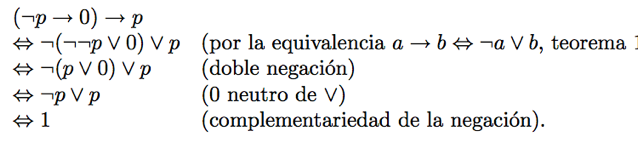
\includegraphics[width=.85\textwidth]{imagenes/apendices/APENDICESIM31.png}
	\end{figure}


Por último, la prueba de uno de los razonamientos que involucran cuantificadores y enunciados abiertos. Probamos el razonamiento de especificación universal usando uno de los razonamientos lógicos de este mismo teorema, supuesto ya demostrado. La proposición $\forall x, p(x)$ es equivalente a la conjunción de la proposición $p(x)$ cuando $x$ toma todos los valores posibles. Entonces, por la regla de simplificación conjuntiva, de la premisa deducimos que cualquiera de las proposiciones es cierta, en particular, si $a$ es un valor posible de $x$, $p(a)$ es cierta.

\rightline{$\Box$}

\vspace{5mm}\textbf{6. Axiomas, definiciones y teoremas en matemáticas}

La matemática deduce resultados nuevos a partir de otros ya conocidos usando la herramienta de la lógica. Una teoría matemática se compone de axiomas, definiciones y teoremas, así que veamos qué es cada uno de ellos.

\underline{\textbf{Axiomas}}: Son las proposiciones de partida de una teoría y, por tanto, no pueden ser probadas dentro de ella. La idea es que los axiomas van a ser las primeras premisas que permitan deducir consecuencias de ellas, es decir, obtener los primeros resultados. Es claro que toda teoría que se construya mediante razonamientos lógicos debe tener axiomas, ya que los razonamientos parten de premisas ciertas para deducir una consecuencia cierta. Es decir, en todo caso necesitamos partir de algunas premisas.

\underline{Ejemplo}: La proposición “el conjunto N de los números naturales contiene al menos un elemento” se utiliza como axioma en la construcción de los números debida a \emph{Peano}.

\underline{\textbf{Definición}}: Es la asignación de un nombre a una proposición y por ello tiene forma de equivalencia. Obsérvese que el papel de las definiciones en una teoría matemática no es determinante, pues sólo sirven para simplificar la escritura (aunque ciertamente sería impensable escribir una teoría sin la ayuda de las definiciones). Es interesante hacer notar que, por ser una equivalencia, una definición debería leerse “. . . si y sólo si . . . ”, sin embargo es costumbre escribir únicamente “...si ...” como si se tratara de una implicación, aún sabiendo que es algo más.

\underline{Ejemplo}: La proposición “un número natural es primo si (y sólo si) es mayor que 1 y sus únicos divisores son $1$ y él mismo” es una definición. Simbólicamente: 

\hspace{2cm} $p$ primo $\Leftrightarrow p>1 \wedge  \forall n , (\,(n|p \to (n=1 \vee n=p)\, )$

Sirve para sustituir en cualquier punto de la teoría la proposición: 
``$p>1 \wedge  \forall n , (\,(n|p \to (n=1 \vee n=p)\, )$'' 
por la otra parte más breve: ``$p$ es primo''.

\underline{\textbf{Teoremas}}: Son los resultados de la teoría y, por tanto, el objetivo de las matemáticas. Son proposiciones que pueden tener diversas formas. Un tipo habitual de teorema es un razonamiento lógico, de la forma descrita anteriormente ``$ p1 \wedge p2 \wedge \cdots \wedge pn \Rightarrow  q$'', en el cual las premisas son los axiomas de la teoría o bien otros teoremas ya probados en la teoría. La consecuencia es otra proposición relativa a la teoría.

\underline{Ejemplo}: El resultado “si $m$ y $n$ son primos distintos, entonces su máximo común divisor es $1$” es un teorema, que podemos escribir también como:

\hspace{2cm} $m \text{ primo } \wedge n \text{ primo } \wedge m \neq n \Rightarrow mcd(m,n)=1.$

Otros teoremas tienen forma de equivalencia ($ \Leftrightarrow $) en lugar de implicación ($\Rightarrow $ ). Pero, como se ha visto anteriormente, un teorema de doble implicación equivale a dos teoremas de una implicación. Esto es, un teorema de la forma $p \Leftrightarrow  q$ es equivalente a $(p \Rightarrow q) \wedge (q \Rightarrow p)$.

\emph{Todo teorema de una teoría debe ser probado rigurosamente}.

Por tanto, la exposición de una teoría matemática debe observar dos reglas imprescindibles: un estricto orden de presentación, para que cada teorema use como premisas sólo resultados anteriores, ya probados, y que cada teorema vaya seguido inmediatamente de su demostración, que consiste en verificar el razonamiento lógico.

Es conveniente señalar que, en ocasiones, se dan otros nombres a resultados de la teoría. Algunos nombres muy utilizados son los de \emph{proposición, lema y corolario}. Todos ellos son sinónimos de teorema en cuanto a que son resultados de la teoría. Los distintos nombres se utilizan para agrupar los resultados por categorías. Una proposición es un resultado de no mucha importancia. Se suele llamar lema a un resultado cuya única aplicación es en la prueba de algún otro resultado posterior. La palabra teorema se reserva para los resultados más importantes de la teoría. Por último, corolario es un resultado cuya prueba es inmediata a partir de un teorema anterior. Como se puede apreciar, llamar a los resultados de una teoría teoremas, lemas, proposiciones o corolarios es una cuestión subjetiva que queda a gusto del autor en cada caso.

\textbf{Un ejemplo}.

A continuación construimos un ejemplo de un desarrollo matemático. Introducimos algunos elementos de la teoría de la divisibilidad de números naturales con el formato explicado: axiomas, definiciones, teoremas y su demostración. En concreto ilustramos un axioma de los naturales, el de inducción, y cuatro teoremas demostrando cada uno con un estilo de prueba diferente: una prueba de la implicación directa, una prueba usando la implicación contrapositiva, una prueba por inducción y una prueba por contradicción.

Para estos ejemplos asumimos conocidas las propiedades algebraicas de la suma y el producto de los naturales como son la asociatividad, conmutatividad o propiedad distributiva o que $n + 1$ es el sucesor del número $n$.

\underline{Axioma}: (\emph{Axioma de inducción de los naturales}). Si el natural $1$ verifica una propiedad y para cada natural $n$ que cumple dicha propiedad también el sucesor de $n$ la cumple, entonces la propiedad se verifica para todos los naturales. Simbólicamente, si $p(x)$ es un enunciado abierto y la variable $x$ toma valores en los naturales, $p(1) \wedge \forall n , (p(n) \to  (\,p(n + 1)\,) \Rightarrow \forall x, p(x)$

\underline{Definición}: Un natural $a$ divide a otro $b$, y lo denotamos $a|b$, si existe un número $c$ tal que se verifica $b = a \cdot c$. Es decir, $a|b \Leftrightarrow \exists c,\;  b = a \cdot c$

En tal caso decimos que $a$ es divisor de $b$ y que $b$ es múltiplo de $a$.

\underline{Ejemplo}: $3|12$ pues $12 = 3 \cdot 4$, pero $5 \cancel{|} 12$ (que es la negación de $5|12$).

Es obvio que $1$ divide a cualquier número $b$ ya que $b = 1b$ y, por la misma razón, todo número es divisor de sí mismo. Algunos números únicamente tienen estos divisores y por ello merecen especial atención.

\underline{Definición}: Un natural $p$ mayor que $1$ es \emph{primo} si $1$ y $p$ son sus únicos divisores. Simbólicamente: $p \text{ primo } \Leftrightarrow p>1 \wedge \forall a, (\, a|p \to a=1\,  \vee \, a=p \,)$. Un natural mayor que $1$ que no es primo se llama compuesto.

\underline{Ejemplo}: Los números primos menores que $100$ son: $2, 3, 5, 7, 11, 13, 17, 19, 23, 29, 31, 37, 41, 43, 47, 53, 59, 61, 73, 79, 83, 89, 97$.

\underline{Teorema}: (\emph{Propiedad transitiva de los divisores}). Si $a$ divide a $b$ y éste, a su vez, divide a $c$, entonces $a$ divide a $c$, que lo podemos escribir como: $(a|b) \wedge (b|c) \Rightarrow  (a|c)$

\underline{Demostración}: Se trata de un teorema con forma de implicación y mostramos una prueba directa, es decir, que partiendo de las premisas y resultados anteriores (propiedades de los números naturales), llegamos a la conclusión mediante las reglas de inferencia enumeradas en un teorema anterior.

\begin{itemize}
	
\item 1. Por hipótesis $a|b$ 

\item 2. Por definición y por la regla de especificación existencial, existe un número, y lo llamamos $k_1$, que cumple $b = k1\cdot a$ 

\item 3. Por hipótesis $b|c$ 

\item 4. Por definición y por la regla de especificación existencial, existe un número, y lo llamamos $k_2$, que cumple $c = k_2 \cdot b$ 

\item 5. Sustituyendo la igualdad del punto 2 en la del punto 4 tenemos $c = k_2 \cdot (k_1 \cdot a)$

\item 6. Por la propiedad asociativa del producto de números naturales la igualdad anterior se puede escribir como $c = (k_2\, k_1)\, a$

\item 7. El número $k_2\, k_1$ hace que se verifique la definición de divisibilidad para $a$ y $c$, luego concluimos que $a$ divide a $c$ 
\end{itemize}

\rightline{$\Box$}

\underline{Teorema} El natural $a$ divide a $b$ sólo si $a$ es menor o igual que $b$. Simbólicamente: $a|b \Rightarrow a 	\le  b$

\underline{Demostración}: Este teorema tiene de nuevo la forma de una implicación, pero ahora vamos a probar la implicación contrapositiva, que es equivalente a la enunciada:  $a > b  a \cancel{|} b$. Ahora los pasos para demostrar ésta.
\begin{itemize}
\item 1. Por hipótesis $a > b$ 

\item 2. Consideremos un natural arbitrario $c$ 

\item 3. Por las propiedades del orden de los naturales $c \ge  1$ 

\item 4. Por las propiedades del orden de los naturales $a\cdot c \ge  a$ 

\item 5. Por los puntos 4 y 1 y las propiedades del orden tenemos $a \cdot c > b$, y por tanto, $a\cdot c \neq  b$ 

\item 6. Por generalización universal, teniendo en cuenta el punto 2, tenemos  $\forall  x,\,   a \cdot x  \neq b$ 

\item 7. La proposición anterior es equivalente a $ \; \neg \exists x\, ,\,  a \cdot x = b$ 

\item 8. Por definición llegamos a   $a \cancel{|} b$ y la implicación contrapositiva queda probada.
\end{itemize}

\rightline{$\Box$}

\underline{Teorema}: Todo número natural cumple que, o bien es $1$, o bien es divisible por un primo, y lo expresamos como sigue  $\forall n,\;   n=1 \; \vee \; \exists p,\, (\, p \text{ primo } \; \wedge \;  p|n\, )$

\underline{Demostración} Aquí presentamos una típica prueba por inducción, que hace uso del axioma del mismo nombre. Para probar que la propiedad enunciada en el teorema es válida para todos los naturales hay que probar que se cumple para el $1$ y que para todo número $n$ que la verifica, la propiedad es válida para el sucesor. Al asumir que se cumple para un número $n$ se puede asumir también que se cumple para todos los menores a él.

\begin{itemize}
	
\item 1. Llamamos $P (n)$ al enunciado $n=1 \; \vee \; \exists p,\, (\, p \text{ primo } \; \wedge \;  p|n \,)$

\item 2. La proposición $P (1)$ es cierta, ya que se cumple $1 = 1$ 

\item 3. Para probar $P (n) \to  P (n + 1)$ consideramos un número $n$ arbitrario y la hipótesis $P (n)$. Entonces el número $n$, si no es $1$, es divisible por un primo y lo mismo cumplen todos los números menores que $n$. Puesto que el número $n+1$ no puede ser $1$, hay que probar que es divisible por un primo. Separamos esta parte en dos casos. 

\item 4. Si $n + 1$ es primo entonces, puesto que $(n + 1)|(n + 1)$, es divisible por un primo y la proposición $P (n + 1)$ es cierta. 

\item 5. Si $n + 1$ no es primo entonces, por definición, tiene un divisor diferente de $1$ y de sí mismo. Por la regla de especificación existencial llamamos $a$ a este divisor.

\item 6. Por teorema, $a < n+1$

\item 7. Por conjunción de los puntos 5 y 6 tenemos  $a  \neq 1 \, \wedge \, a<n+1$

\item 8. Por la hipótesis de inducción (punto 3) aplicada al número $a$, y por la regla de especificación existencial, existe un número primo, y lo llamamos $p$, que cumple $p|a$

\item 9. Por conjunción de los puntos 5 y 8 tenemos $p|a \; \wedge \;  a|(n + 1)$. Usando el teorema  concluimos $p|(n + 1)$, es decir $P (n + 1)$ es cierta también en este caso.

\item 10. Por la regla de inferencia de demostración por casos aplicada a los puntos 4 y 10 concluimos que $ \forall n,\,  P (n) \to  P (n + 1)$ es cierta.

\item 11. Por conjunción de los puntos 2 y 11 y el axioma llegamos a que el enunciado $P(n)$ es cierto para todos los naturales, luego el teorema queda probado.

\end{itemize}
\rightline{$\Box$}


Por último enunciamos un famoso teorema y su, no menos famosa, prueba debida a Euclides: la infinitud de los números primos y su demostración por contradicción.



\underline{Teorema}: (\emph{Euclides}). La cantidad de números primos es infinita. 

\underline{Demostración}: Aquí presentamos la prueba debida a Euclides, que procede por contradicción o, como también se llama, reducción al absurdo.

\begin{itemize}
	
\item 1. Negamos el teorema: La cantidad de números primos es finita. 

\item 2. Por ser finita, podemos denotar los números primos como $p_1, p_2, \cdots, p_n$. 

\item 3. Consideremos el número $q = p_1 \cdot  p_2 \cdot  \cdots \cdot  p_n \, + \, 1$ 

\item 4. Por su construcción y las propiedades del orden de los naturales $q > 1$, por lo cual $q \neq 1$ 

\item 5. En este punto demostramos que $p_1$ no divide a $q$ utilizando también un razonamiento por contradicción: negamos la afirmación, asumiendo entonces que $p_1$ sí divide a $q$. Entonces $q = p_1\cdot k$ para algún número $k$ y, operando en la definición de $q$, podemos escribir $1 = p1\,(k - p_2 \cdot p_3 \cdot \cdots \cdot  p_n)$. Esta igualdad indica que $p_1$ divide a $1$. 

\item 6. Por un teorema anterior tenemos que $p1 \le 1$. Sin embargo, por hipótesis $p_1$ es primo y, por  definición, esto supone $p_1 > 1$. Tenemos la contradicción $p1 \le 1 \; \wedge \;  p1 > 1$. Por tanto concluimos que la negación es falsa y queda probado que $p_1 \cancel{|}q$. Análogamente tenemos $p_2 \cancel{|}q, \cdots  p_n \cancel{|}q$ 

\item 7. Por conjunción de los dos puntos anteriores tenemos que el número $q$ no es $1$ y no es divisible por ningún primo, lo cual es una contradicción con el teorema.

\item 8. Por la regla de contradicción concluimos que el enunciado original es cierto.
\end{itemize}
\rightline{$\Box$}

Las demostraciones que aquí se han puesto como ejemplo han sido ilustradas con mucho detalle, pero habitualmente la redacción de pruebas de teoremas se hace mucho más breve. Las cuatro pruebas anteriores, en un lenguaje habitual, se reducirían a unas pocas líneas cada una, especialmente porque no se mencionan las reglas de inferencia que se usan en cada paso ya que son ampliamente conocidas.


\clearpage


 INVESTIGA: ALGEBRA DE BOOLE DE:

\small{\hspace{1cm} --PROPOSICIONES LÓGICAS} 

\small{\hspace{1cm} --CONJUNTOS}

\small{\hspace{1cm} --CIRCUITOS ELEÉCTRICOS}
	
	\begin{figure}[H]
		\centering
		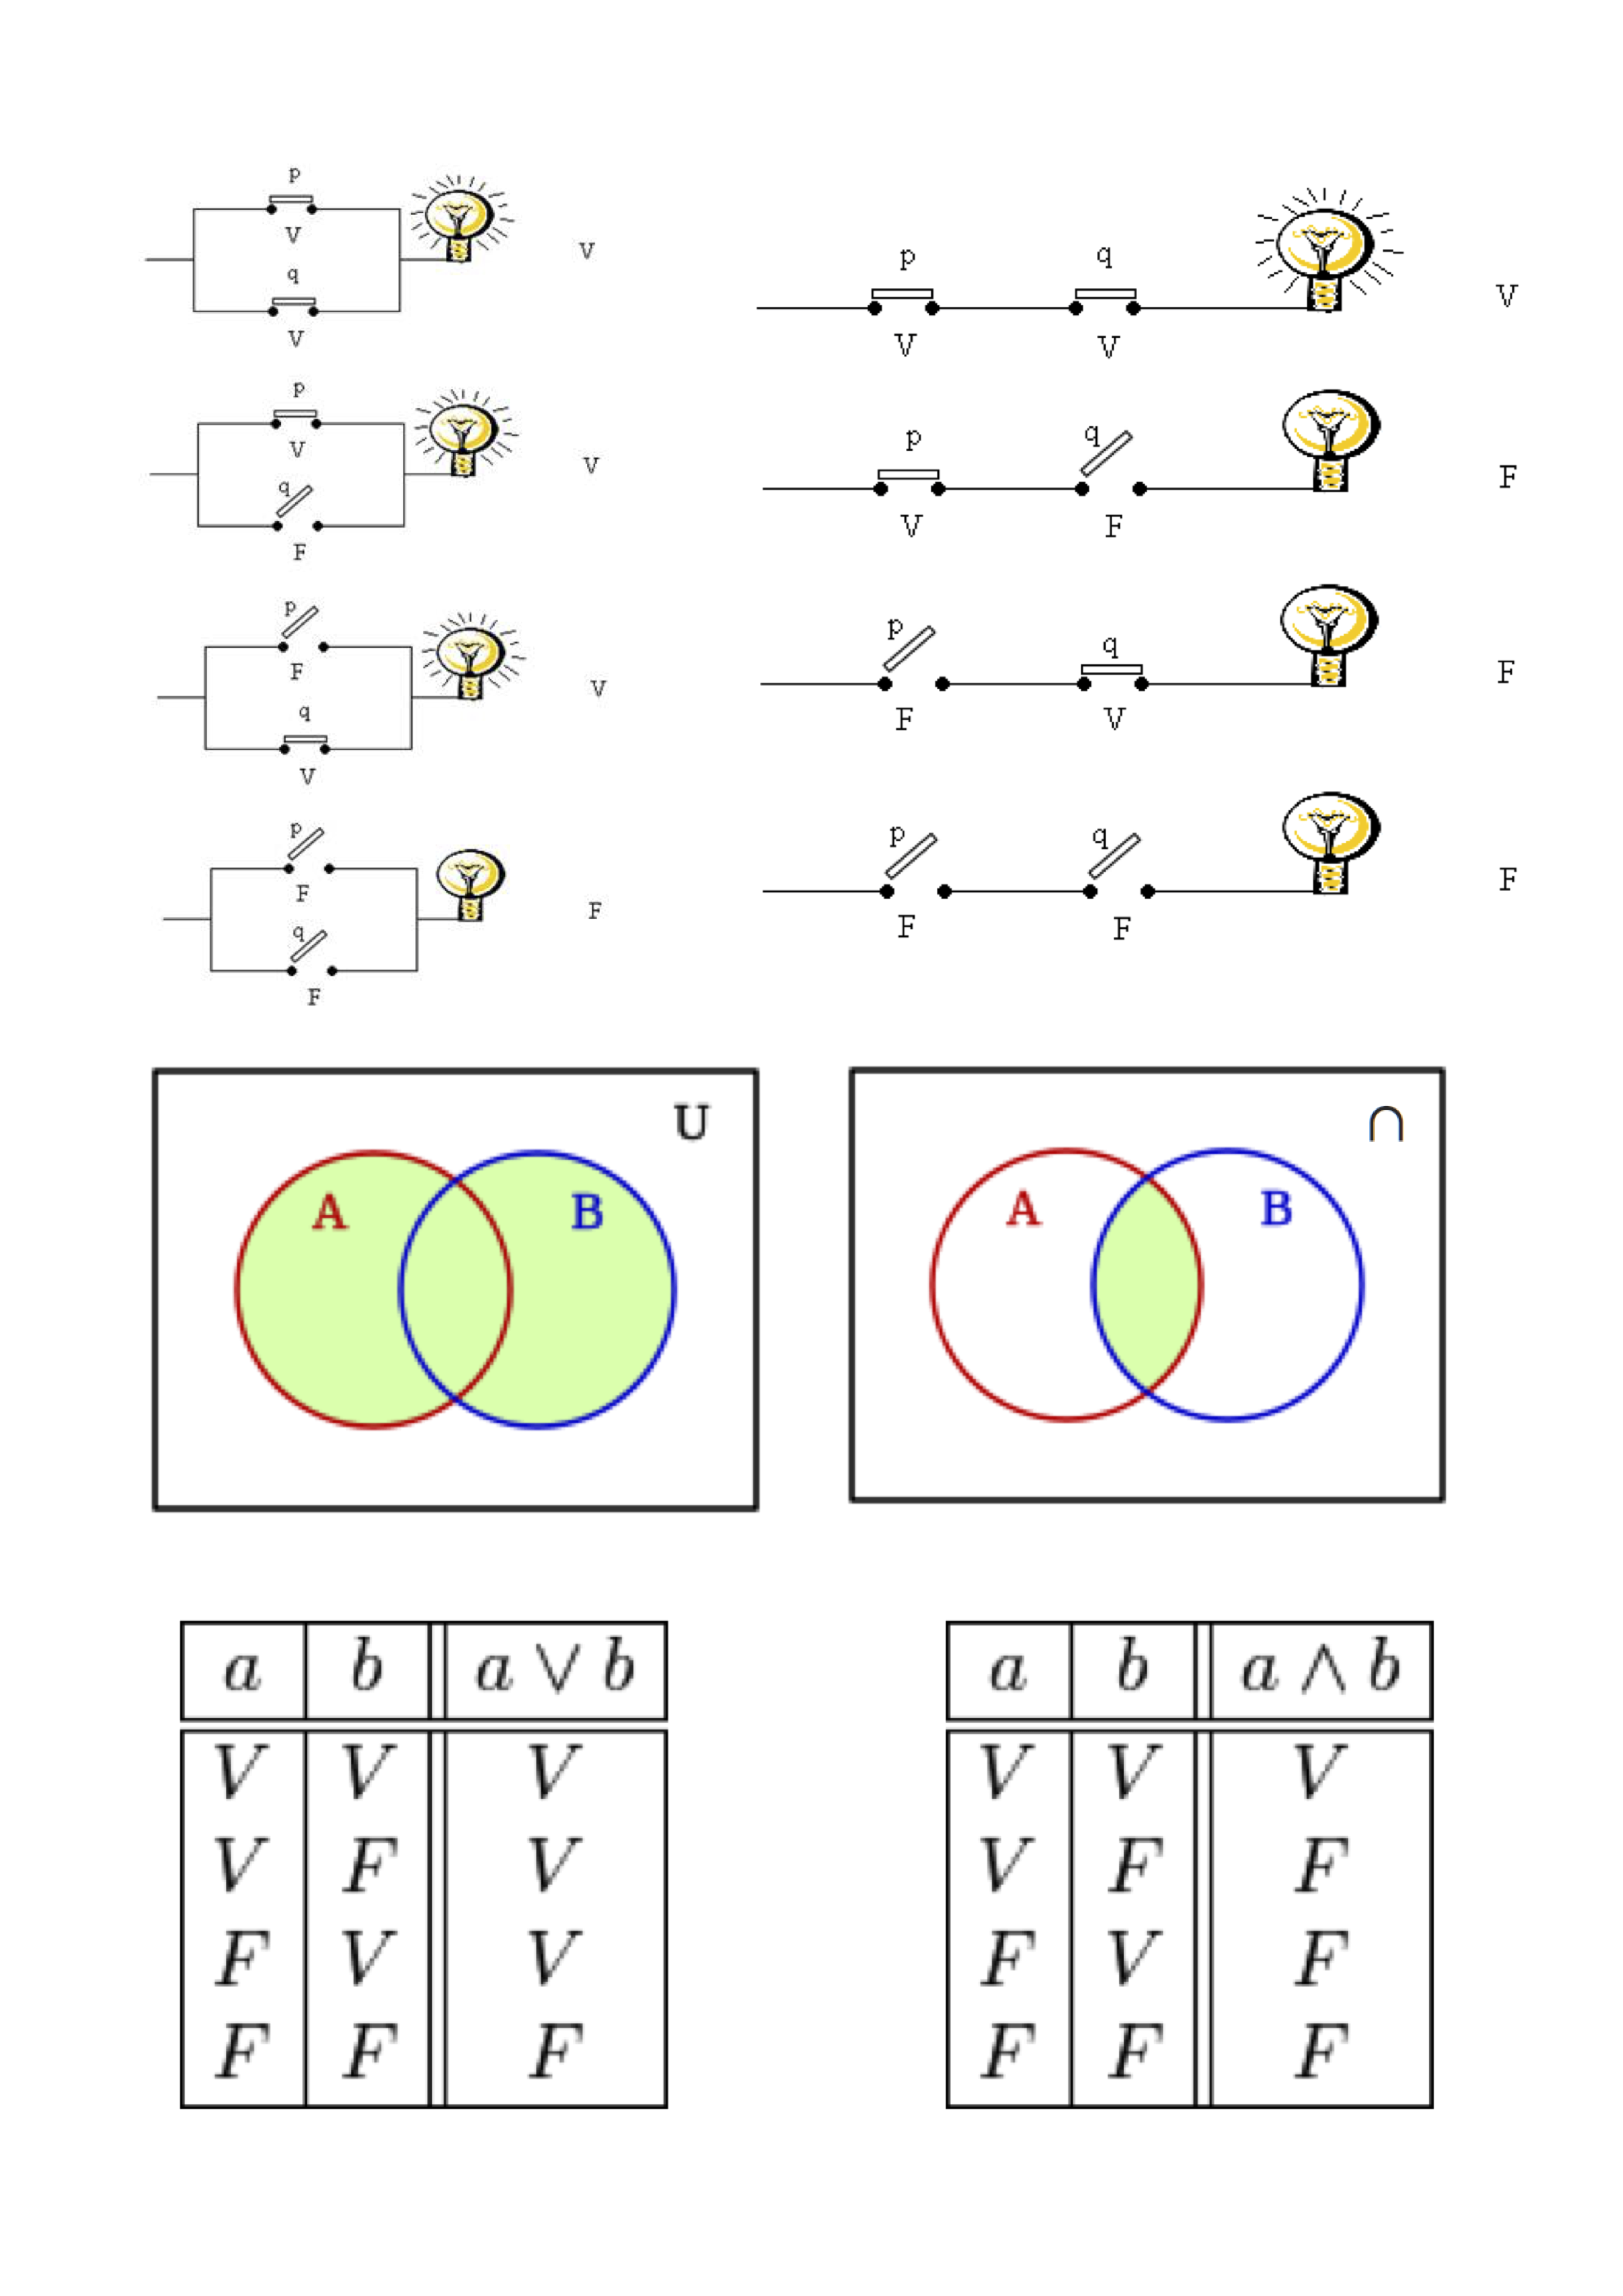
\includegraphics[width=0.9\textwidth]{imagenes/apendices/APENDICESIM32.png}
	\end{figure}    
	
	
	
	
	

\chapter{\small{Gráficas de las funciones elementales más conocidas}}
\vspace{-10mm}
\begin{figure}[H]
		\centering
		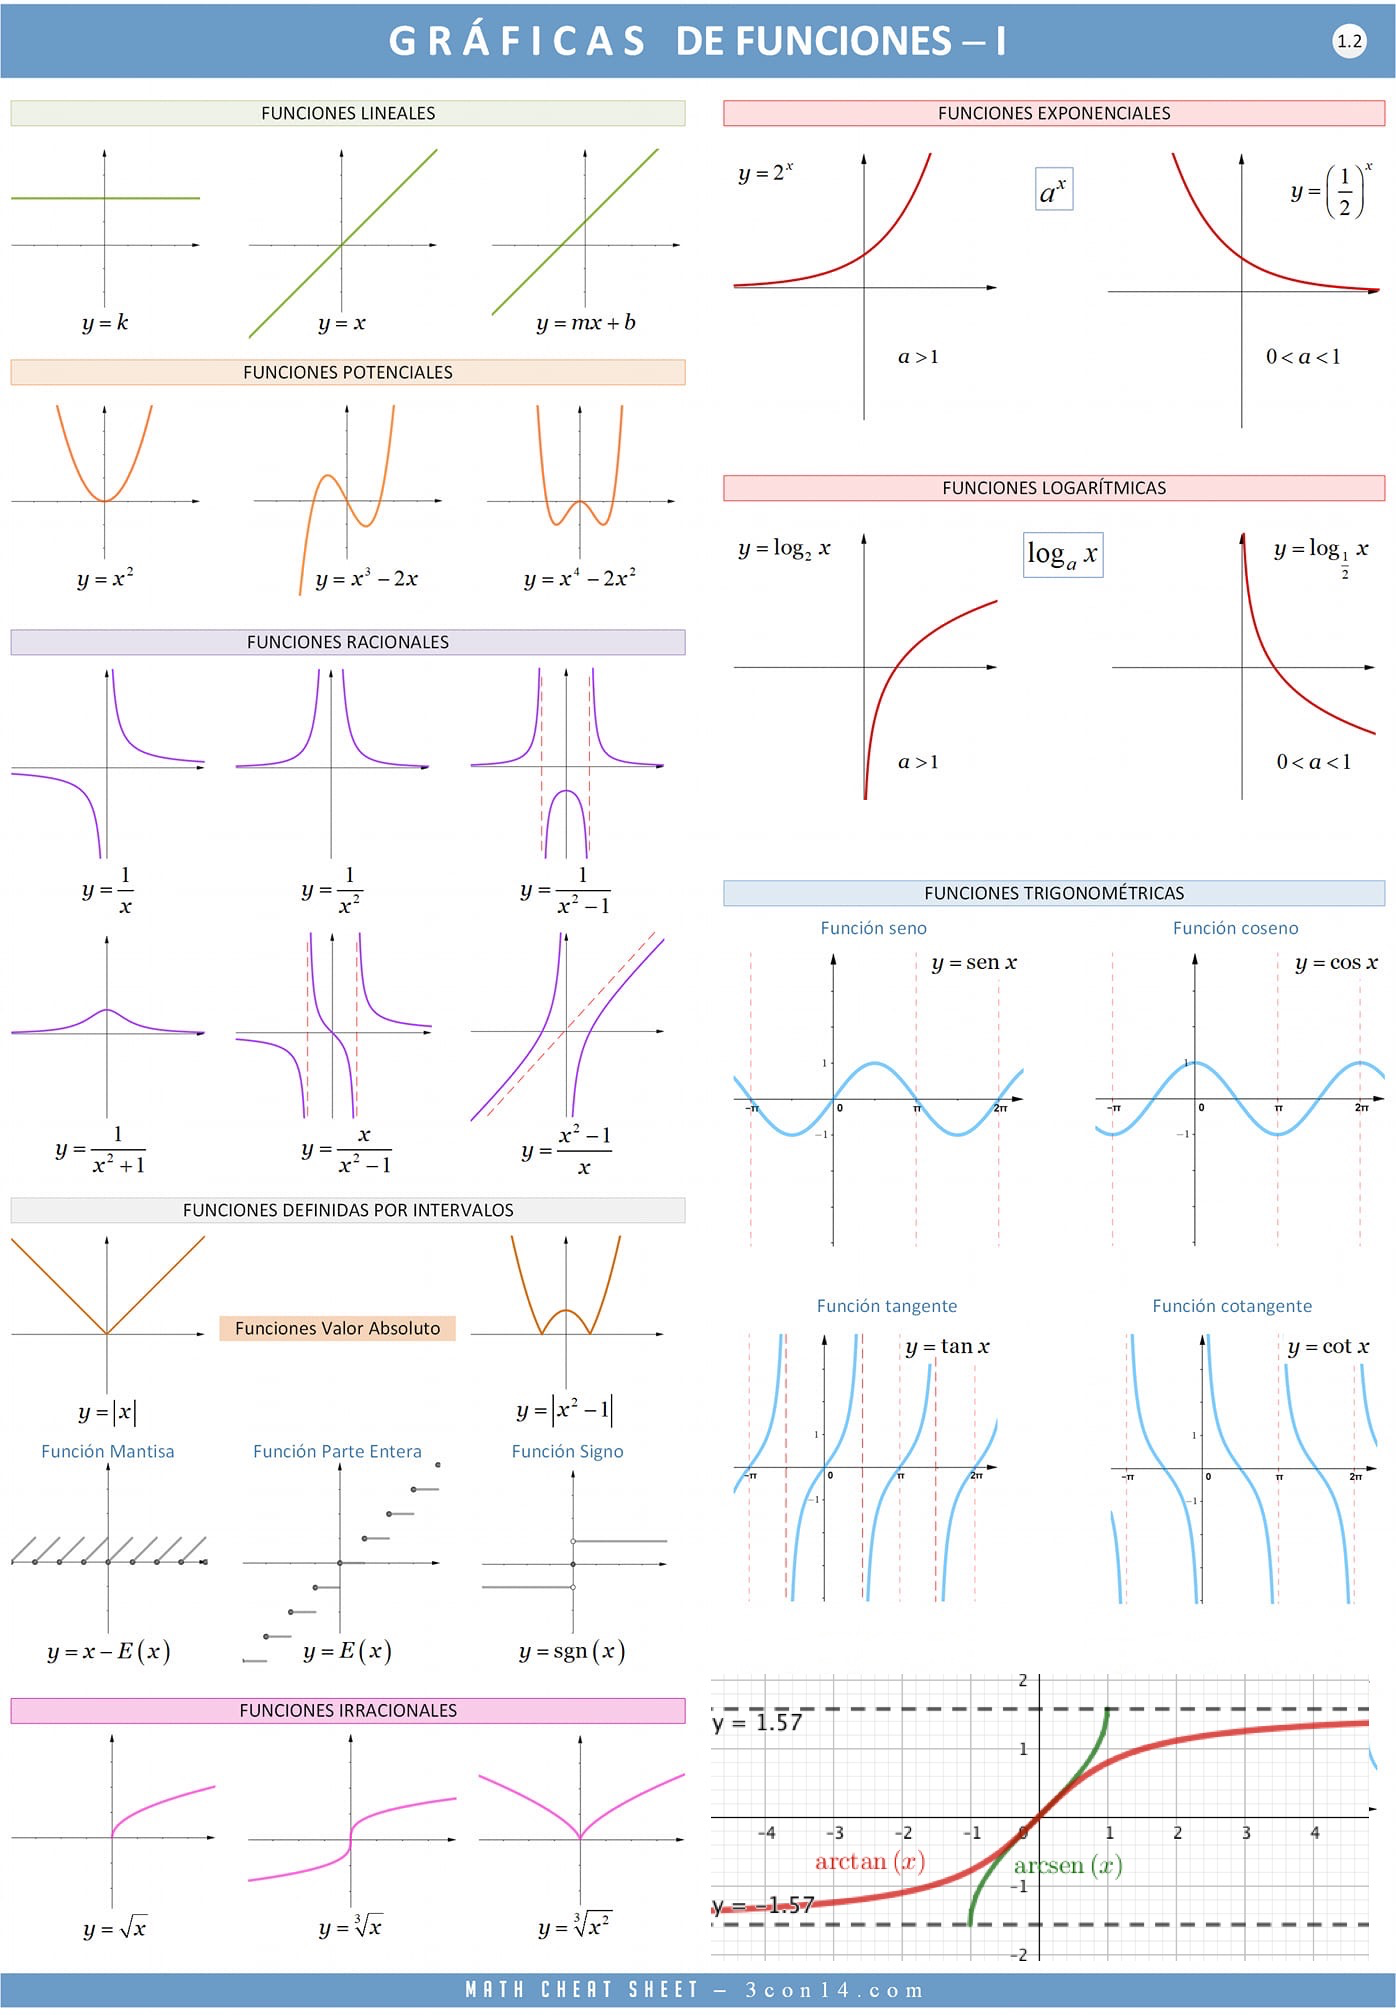
\includegraphics[width=0.85\textwidth]{imagenes/apendices/APENDICESIM09.png}
	\end{figure} 
	
	
	
\chapter{Tabla de derivadas}
	\label{app:tabla-derivadas}
	%\vspace{-10mm}

	\begin{table}[H]
	\centering
	\def\arraystretch{1.6}
	\begin{tabular}{|l|l|l|l|}
	\hline
	\multicolumn{4}{|c|}{TABLA DE DERIVADAS} \\ \hline
	\multicolumn{2}{|l|}{Funciones elementales} & \multicolumn{2}{l|}{Funciones compuestas} \\ \hline
        $f(x)=k$   &  $f'(x)=0$         &           &           \\ \hline
        $f(x)=x$   & $f'(x)=1$          &           &           \\ \hline
         $f(x)=x^n$  & $f'(x)=n\; x^{n-1}$          & $f(x)=u^n$          &   $f'(x)=n\; u^{n-1} \cdot u'$        \\ \hline
          $f(x)=\dfrac 1 x$  & $f'(x)=-\dfrac 1 {x^2}$    & $f(x)=\dfrac 1 u$    &  $f'(x)=-\dfrac 1 {u^2} \cdot u'$  \\ \hline
        $f(x)=\sqrt{x}$    & $f'(x)=\dfrac {1}{2\sqrt{x}}$    &    $f(x)=\sqrt{u}$ & $f'(x)=\dfrac {1}{2 \sqrt{u}} \cdot u'$   \\ \hline
       $f(x)=\ln x$    & $f'(x)=\dfrac 1 x$    & $f(x)=\ln u$    & $f'(x)=\dfrac {u'}{u}$   \\ \hline
        $f(x)=\log_a x$   & $f'(x)=\dfrac {1}{x\; \ln a}$    &  $f(x)=\log_a u$   & $f'(x)=\dfrac {1}{u \; \ln a} \cdot u'$   \\ \hline
         $f(x)=e^x$  & $f'(x)=e^x$    & $f(x)=e^u$    & $f'(x)=e^u \cdot u'$   \\ \hline
         $f(x)=a^x$  & $f'(x)=a^x \; \ln a$    & $f(x)=a^u$    & $f'(x)=a^u \; \ln a \cdot u'$   \\ \hline
        $f(x)=\sin x$   & $f'(x)=\cos x$    & $f(x)=\sin u$    & $f'(x)=\cos u \cdot u'$    \\ \hline
           $f(x)=\cos x$   & $f'(x)=-\sin x$    & $f(x)=\cos u$    & $f'(x)=-\sin u \cdot u'$    \\ \hline
       $f(x)=\tan x$    & \scriptsize{$f'(x)=\dfrac 1 {\cos^2 x}=1 +\tan^2 x$}  &  $f(x)=\tan u$ &  \scriptsize{$f'(x)=\dfrac 1 {\cos^2 u} \cdot u'=(1 +\tan^2 u)\cdot u'$ }       \\ \hline
       $f(x)=\arcsin x$    & $f'(x)=\dfrac {1}{\sqrt{1-x^2}}$    &    $f(x)=\arcsin u$   & $f'(x)=\dfrac {1}{\sqrt{1-u^2}}\cdot u'$   \\ \hline
        $f(x)=\arccos x$    & $f'(x)=\dfrac {-1}{\sqrt{1-x^2}}$    &    $f(x)=\arccos u$   & $f'(x)=\dfrac {-1}{\sqrt{1-u^2}}\cdot u'$   \\ \hline
       $f(x)=\arctan x$    & $f'(x)=\dfrac {1}{1+x^2}$    &    $f(x)=\arctan u$   &   $f'(x)=\dfrac {1}{1+u^2} \cdot u'$  \\ \hline        
	\end{tabular}
	\end{table}
	
	
	
	
	\begin{table}[H]
	\centering
	\def\arraystretch{1.6}
	\begin{tabular}{|l|l|l|l|}
	\hline
	\multicolumn{4}{|c|}{TABLA DE DERIVADAS (continuación)} \\ \hline
	\multicolumn{2}{|l|}{Funciones elementales} & \multicolumn{2}{l|}{Funciones compuestas} \\ \hline
        $f(x)=k$   &  $f'(x)=0$         &           &           \\ \hline
        $f(x)=x$   & $f'(x)=1$          &           &           \\ \hline
         
         $\divideontimes$  $f(x)=\sinh x$ & $f'(x)=\cosh x$    &    $f(x)=\sinh u$  & $f'(x)=\cosh u \cdot u'$   \\ \hline
         $\divideontimes$  $f(x)=\cosh x$ & $f'(x)=\sinh x$    &    $f(x)=\cosh u$  & $f'(x)=\sinh u \cdot u'$   \\ \hline
         $\divideontimes$ $f(x)=\tanh x$   & $f'(x)=1-\tanh^2 x$    &  $f(x)=\tanh u$   &   $f'(x)=(1-\tanh^2 u) \cdot u'$  \\ \hline
         $\divideontimes$ $f(x)=\mathrm{arg sinh} \;x$   & $f'(x)=\dfrac {1}{\sqrt{x^2+1}}$    & $f(x)=\mathrm{arg sinh} \; u$   &   $f'(x)=\dfrac {1}{\sqrt{u^2+1}}\cdot u'$  \\ \hline
         $\divideontimes$ $f(x)=\mathrm{arg cosh} \; x$   & $f'(x)=\dfrac {1}{\sqrt{x^2-1}}$    & $f(x)=\mathrm{arg cosh} \; u$   &   $f'(x)=\dfrac {1}{\sqrt{u^2-1}}\cdot u'$  \\ \hline
         $\divideontimes$ $f(x)=\mathrm{arg tanh} \; x$   & $f'(x)=\dfrac {1}{x^2-1}$    & $f(x)=\mathrm{arg tanh} \; u$   &   $f'(x)=\dfrac {1}{1-u^2}\cdot u'$  \\ \hline
               
               
               
	\end{tabular}
	\end{table}
	
\chapter{Desarrollos en serie de Maclaurin de las funciones más usadas}	\label{tabla-maclaurin}

\begin{itemize}
	\item $e^x=1+x+\dfrac{x^2}{2!}+\dfrac{x^3}{3!}+\dfrac{x^4}{4!}+\cdots \qquad -\infty < x < +\infty$
	\item $\mathrm{ln}\; (1+x)=x-\dfrac{x^2}{2}+\dfrac{x^3}{3}-\dfrac{x^4}{4}+\dfrac{x^5}{5}- \cdots \qquad -1 < x \le 1 $
	
	\textcolor{gris}{\small{Para $\mathrm{ln}\; x$, sustituir $1+x \mbox{ por } x$, así, el desarrollo sería válido en $0<x\le 2$}}
	\item $\dfrac{1}{1+x}=1-x+x^2-x^3+x^4-x^5+\cdots \qquad -1<x<1$
	
	\textcolor{gris}{\small{Para $\dfrac {1}{1-x}$, sustituir $x \mbox{ por } -x$, así, el desarrollo sería válido también en $-1<x< 1$}}
	\item $(1+x)^r=\left( \begin{matrix} r \\ 0 \end{matrix} \right) +\left( \begin{matrix} r \\  \end{matrix} \right) x+\left( \begin{matrix} r \\ 2 \end{matrix} \right) x^2+\left( \begin{matrix} r \\ 3 \end{matrix} \right) x^3+\cdots =\sum _{ k=0 }^{ n }{ \left( \begin{matrix} r \\ k \end{matrix} \right) { x }^{ k } } \qquad -1<x<1$
	
	\item $\sqrt{1+x} = 1 + \dfrac 1 2 x -\dfrac 1 {24} x^2 + \dfrac {13}{246}x^3- \cdots \qquad -1<x\le 1 $
	\item $\sin x = x -\dfrac{x^3}{3!}+\dfrac{x^5}{5!}-\dfrac{x^7}{7!}+\cdots \qquad -\infty < x < +\infty$
	\item $\cos x = 1 -\dfrac{x^2}{2!}+\dfrac{x^4}{4!}-\dfrac{x^6}{6!}+\cdots \qquad -\infty < x < +\infty$
	\item $\tan x= x+ \dfrac{x^3}{3}+\dfrac{2x^5}{15}+\dfrac{17x^7}{315}+\dfrac{62x^9}{2835}+ \cdots \qquad x^2<\pi^2/4$
	\item $\arcsin x =x+\dfrac{x^3}{2 \cdot 3}+\dfrac{1\cdot 3}{2 \cdot 4\cdot 5}x^5+\dfrac{1\cdot 3 \cdot 5}{2\cdot 4 \cdot 6 \cdot 7}x^7+ \cdots \qquad x^2<1$
	\item $\arccos x = \dfrac {x}{2}- \left[ \dfrac{x^3}{2 \cdot 3}+\dfrac{1\cdot 3}{2 \cdot 4\cdot 5}x^5+\dfrac{1\cdot 3 \cdot 5}{2\cdot 4 \cdot 6 \cdot 7}x^7+ \cdots \right] \qquad x^2<1$
	\item $\arctan x=x - \dfrac {x^3}{3} +\dfrac {x^5}{5}-\dfrac {x^7}{7}+\cdots \qquad x^2<1$

	
\end{itemize}
	

\chapter{Tabla de integrales}
\label{app:tabla-integrales}
\begin{table}[H]
\centering
\def\arraystretch{2}
\begin{tabular}{|c|c|}
\hline
\multicolumn{2}{|c|}{Tabla de integrales inmediatas} \\ \hline
      \emph{Función elemental} & 	\emph{Función compuesta}      \\ \hline
  $\displaystyle \int k \; \dd x=kx+\mathcal{C}$    &  $\quad$        \\ \hline
   $\displaystyle \int x^n \; \dd x = \dfrac {x^{n+1}}{n+1} +\mathcal{C}; \; n\neq -1$         &   $\displaystyle \int f'\cdot  f^n \; \dd x = \dfrac {f^{n+1}}{n+1} +\mathcal{C}; \; n\neq -1$          \\ \hline
     $\displaystyle \displaystyle \int {\dfrac 1 x \; \dd x} = \mathrm{ln}|x|+\mathcal{C}$      &     $\displaystyle \displaystyle \int {\dfrac {f'} {f} \; \dd x} = \mathrm{ln}|f|+\mathcal{C}$       \\ \hline
 $\displaystyle \int e^x\; \dd x= e^x +\mathcal{C}$          &    $\displaystyle \int f' \cdot  e^f\; \dd x= e^f +\mathcal{C}$         \\ \hline
  $\displaystyle \int a^x\; \dd x= \dfrac {a^x}{\mathrm{ln}a} +\mathcal{C}$          &    $\displaystyle \int f' \cdot  a^f\; \dd x= \dfrac{e^f}{\mathrm{ln}a} +\mathcal{C}$         \\ \hline
  $\displaystyle \int \sin x \; \dd x= - \cos x + \mathcal{C}$         &  $\displaystyle \int f'\cdot \sin f \; \dd x= - \cos f + \mathcal{C}$           \\ \hline
    $\displaystyle \int \cos x \; \dd x=\sin x + \mathcal{C}$         &  $\displaystyle \int f'\cdot \cos f \; \dd x= \sin f + \mathcal{C}$           \\ \hline
     $\displaystyle \int \sinh x \; \dd x=  \cosh x + \mathcal{C}$         &  $\displaystyle \int f'\cdot \sinh f \; \dd x= \cosh f + \mathcal{C}$           \\ \hline
        $\displaystyle \int \cosh x \; \dd x=  \sinh x + \mathcal{C}$         &  $\displaystyle \int f'\cdot \cosh f \; \dd x= \sinh f + \mathcal{C}$           \\ \hline
    $\displaystyle \int \dfrac {1}{\sqrt{1-x^2}}\; \dd x = \arcsin x + \mathcal{C}$       &      $\displaystyle \int f' \cdot \dfrac {1}{\sqrt{1-f^2}}\; \dd x = \arcsin f + \mathcal{C}$         \\ \hline
     $\displaystyle \int \dfrac {1}{1+x^2}\; \dd x = \arctan x + \mathcal{C}$      &     $\displaystyle \int \dfrac {f'}{1+f^2}\; \dd x = \arctan f + \mathcal{C}$        \\ \hline
\end{tabular}
\end{table}

LINEALIDAD  de la Integral Indefinida:

\begin{equation*}
	 \displaystyle \int \left(a\; f + b \; g \right) \; \dd x =  a \; \displaystyle \int f\; \dd x + b\; \displaystyle \int g \; \dd x
\end{equation*}

\begin{table}[H]
\centering
\def\arraystretch{2}
\begin{tabular}{|c|c|}
\hline
\multicolumn{2}{|c|}{Tabla de integrales inmediatas (ampliación)} \\ \hline
      \emph{Función elemental} & 	\emph{Función compuesta}      \\ \hline
  $\displaystyle \int \dfrac {1}{\cos^2 x} \; \dd = \tan x+\mathcal{C}$    &   $\displaystyle \int f' \cdot \dfrac {1}{\cos^2 f} \; \dd = \tan f+\mathcal{C}$     \\ \hline
    $\displaystyle \int \dfrac {1}{\sin^2 x} \; \dd = \cot x+\mathcal{C}$    &   $\displaystyle \int f' \cdot \dfrac {1}{\sin^2 f} \; \dd = -\cot f+\mathcal{C}$     \\ \hline
    $\displaystyle \int \tan x ; \dd x= -\mathrm{ln}|\cos x|+\mathcal{C}$           &   $\displaystyle \int f'\cdot \tan f ; \dd x= -\mathrm{ln}|\cos f|+\mathcal{C}$       \\ \hline
    $\displaystyle \int \cot x ; \dd x= \mathrm{ln}|\sin x|+\mathcal{C}$           &   $\displaystyle \int f'\cdot \cot f ; \dd x= -\mathrm{ln}|\sin f|+\mathcal{C}$       \\ \hline
      $\displaystyle \int \sec^2 x \; \dd x= \tan x + \mathcal{C}$           &   $\displaystyle \int f' \cdot  \sec^2 f \; \dd x= \tan f + \mathcal{C}$       \\ \hline
        $\displaystyle \int \csc^2 x \; \dd x= -\cot x + \mathcal{C}$           &   $\displaystyle \int f' \cdot  \csc^2 f \; \dd x=- \cot f + \mathcal{C}$       \\ \hline
       $\displaystyle \int \dfrac {\dd x}{\sqrt{x^2 \pm a^2}}  = \mathrm {ln} |x+\sqrt{x^2\pm a^2}|+ \mathcal{C} $       &     $\displaystyle \int \dfrac {f'\cdot \dd x}{\sqrt{f^2 \pm a^2}}  = \mathrm {ln} |f+\sqrt{f^2\pm a^2}|+ \mathcal{C} $      \\ \hline
      $\displaystyle \int \dfrac {\dd x}{\cosh^2 x} = \tanh x + \mathcal{C} $          &    $\displaystyle \int \dfrac {f'\cdot \dd x}{\cosh^2 f} = \tanh f + \mathcal{C} $     \\ \hline
       $\displaystyle \int \dfrac {\dd x}{\sinh^2 x} = -\coth x + \mathcal{C} $          &    $\displaystyle \int \dfrac {f'\cdot \dd x}{\sinh^2 f} = -\coth f + \mathcal{C} $     \\ \hline
         $\displaystyle \int \dfrac {\dd x}{\sqrt{a^2+x^2}}=\mathrm{argsinh} \; \dfrac x a + \mathcal{C} !: a>0$        &    $\displaystyle \int \dfrac {f'\cdot \dd x}{\sqrt{a^2+f^2}}=\mathrm{argsinh} \; \dfrac f a + \mathcal{C} ; a>0$  \\ \hline
           $\displaystyle \int \dfrac {\dd x}{\sqrt{x^2-a^2}}=\mathrm{argcosh} \; \dfrac x a + \mathcal{C} \; a>0; a \neq 1$        &    $\displaystyle \int \dfrac {f'\cdot \dd x}{\sqrt{f^2-a^2}}=\mathrm{argcosh} \; \dfrac f a + \mathcal{C} ; x>a>0$  \\\hline
   \end{tabular}
\end{table}

\chapter{Fin}

	\begin{figure}[H]
		\centering
		\includegraphics[width=.4\textwidth]{imagenes/aleph.png}
	\end{figure}

\vspace{2cm}
 
\rightline{ignaciovallesoriola@gmail.com}

	\begin{figure}[H]
		\raggedleft
		
\includegraphics[width=.4\textwidth]{imagenes/firma.png}
	\end{figure}
